\documentclass[a4paper, 12pt]{article}

\usepackage{cmap}
\usepackage[T2A]{fontenc}
\usepackage[english, russian]{babel}
\usepackage[utf8]{inputenc}
\usepackage[left=2cm,right=1.5cm,top=2cm,bottom=2cm]{geometry}
\usepackage{amsmath}
\usepackage{amssymb}
\usepackage{etoolbox}
\usepackage{amsthm}
\usepackage{booktabs}
\usepackage{graphicx}
\usepackage{tikz}

\newcommand{\Z}{\mathbb{Z}}
\newcommand{\N}{\mathbb{N}}
\newcommand{\R}{\mathbb{R}}
\newcommand{\Q}{\mathbb{Q}}
\newcommand{\B}{\mathfrak{B}}
\newcommand{\Bo}{\mathring{B}}

\renewcommand{\phi}{\varphi}
\renewcommand{\epsilon}{\varepsilon}
\newcommand{\lra}{\Leftrightarrow}
\renewcommand{\emptyset}{\varnothing}
\newcommand\tab[1][.5cm]{\hspace*{#1}}
\newcommand{\lims}{\lim\limits_{n\to \infty}}
\renewcommand{\liminf}{\lim\limits_{x\to \infty}}
\newcommand{\liminfp}{\lim\limits_{x\to +\infty}}
\newcommand{\liminfm}{\lim\limits_{x\to -\infty}}
\newcommand{\lima}{\lim\limits_{x\to a}}
\newcommand{\limo}{\lim\limits_{x\to 0}}
\newcommand{\om}{\bar{\bar{o}}}

\DeclareMathOperator*\lowlim{\underline{lim}}
\DeclareMathOperator*\uplim{\overline{lim}}

\theoremstyle{definition}
\newtheorem*{definition}{Определение}
\newtheorem*{theorem}{Теорема}
\newtheorem*{consequense}{Следствие}
\newtheorem*{lemma}{Лемма}
\newtheorem*{comm}{Замечание}
\newtheorem*{statement}{Утверждение}
\newtheorem*{example}{Пример}
\newtheorem*{examples}{Примеры}
\newtheorem*{axiom}{Аксиома}

\usepackage{titlesec}
\titleformat{\section}{\LARGE \bfseries}{\thesection}{1em}{}
\titleformat{\subsection}{\Large\bfseries}{\thesubsection}{1em}{}
\titleformat{\subsubsection}{\large\bfseries}{\thesubsubsection}{1em}{}

\usepackage{hyperref}
\usepackage{xcolor}
\definecolor{linkcolor}{HTML}{225ae2}
\definecolor{urlcolor}{HTML}{225ae2}
\hypersetup{
    pdfstartview=FitH, 
    linkcolor=linkcolor,
    urlcolor=urlcolor,
    colorlinks=true
}

\title{\textbf{Математический анализ-1}}
\author{Лектор: проф. Подольский Владимир Евгеньевич}

\begin{document}
    \fontsize{14pt}{20pt}\selectfont
    \maketitle
    \vspace{0.3cm}
    \begin{center}
        
\includegraphics[width=0.8\linewidth]{mehmat.png}
    \end{center}
    \vspace{1.5cm}
    \begin{center}
        Конспект: Кирилл Яковлев, 108 группа \tab[5.5cm] tg: @fourkenz
        %Кирилл Яковлев\\
        %группа 108\\
        %\href{https://github.com/yakovlevki}{GitHub}\\
        %\href{t.me/@fourkenz}{Telegram}\\
    \end{center}
    \newpage
    \tableofcontents
    \fontsize{14pt}{20pt}\selectfont
    \newpage

    \section{Элементы теории множеств}
    \subsection{Условности и обозначения}
        \begin{definition}
            Кванторами будем называть символы, заменяющие слова в выражениях.
        \end{definition}
        \begin{comm}
            Пока что кванторы не подразумевают логические операции, мы будем использовать их только для более удобной и формальной записи.
        \end{comm}
        \begin{itemize}
            \item $\forall$ - квантор всеобщности
            \item $\exists$ - квантор существования
            \item $!$ - квантор единственности
            \item Запись $A \Rightarrow B$ обозначает, что из высказывания $A$, следует высказывание $B$. 
            \item Запись $A \lra B$ обозначает, что высказывание $A$ равносильно высказыванию $B$.
            \item Запись $a \in A$ означает, что $a$ является элементом множества $A$, отрицанием такой записи будет $a \notin A$
            \item Если $x$ - объект, а $P$ - свойство, то запись $\{x : P(x)\}$ означает класс всех объектов обладающих свойством $P$.
        \end{itemize}
        \begin{definition}
            Множество, не содержащее ни одного элемента, называется пустым и обозначается $\emptyset$.
        \end{definition}
        \begin{definition}
            Множество $A^{\prime}$ является подмножеством множества $A$, \\ если $\forall a: a\in A^{\prime}\Rightarrow a\in A$. Если $A^{\prime}$ - подмножество A, то пишут $A^{\prime}\subset A$.
        \end{definition}        
        \begin{definition}
            Для любого множества $A$ выполнено:
            \begin{enumerate}
                \item $\emptyset \subset A$.
                \item $A \subset A$.
            \end{enumerate}
        \end{definition}
        \begin{definition}
            Если $A\subset B$ и $A\ne B$, то $A$ называется собственным подмножеством множества $B$.
        \end{definition}
    \subsection{Операции над множествами}
        \begin{definition}
            Множество $C=A\cup B$ называется объединением множеств $A$ и $B$, если $\forall a: (a\in A \Rightarrow a\in C)$ и $\forall b: (b\in B\Rightarrow b\in C)$, а также $\forall c: c\in C \Rightarrow (c\in A$ или $c\in B)$.        \end{definition}
        \begin{definition}
            Множество $C=A\cap B$ называется пересечением множеств $A$ и $B$, если $\forall c: c\in C \Rightarrow (c\in A$ и $c\in B)$, а также $\forall c: (c\in A$ и $c\in B) \Rightarrow c\in C$.        \end{definition}
        \begin{definition}
            Множество $C=A\setminus B$ называется разностью множеств $A$ и $B$, если $\forall c: (c\in A$ и $c\not\in B) \Rightarrow c\in C$, а также $\forall c: c\in C \Rightarrow (c\in A$ и $c\not\in B)$
        \end{definition}
        \begin{statement}
            $A\cup(B\cap C)=(A\cup B)\cap(A\cup C)$.
        \end{statement}
        \begin{proof} 
            $a\in (A\cup(B\cap C)) \lra a\in A$ или $a\in (B\cap C) \lra a\in A$ или $(a\in B$ и $a\in C) \lra (a\in A$ или $a\in B)$ и $(a\in A$ или $a\in C)$.
        \end{proof}
        \begin{statement}
            $A\cap(B\cup C)=(A\cap B)\cup(A\cap C)$.
        \end{statement}
        \begin{proof}
            $a\in (A\cap(B\cup C)) \lra a\in A$ и $a\in (B\cap C)\lra a\in A$ и \\ $(a\in B$ или $a\in C)\lra (a\in A$ и $a\in B)$ или $(a\in A$ и $a\in C)$.
        \end{proof}
    \subsection{Декартово произведение множеств}
        \begin{definition}
            Множество $A$ называется одноэлементным, если $\exists\ a\in A$ такое, что $A\setminus\{a\} = \emptyset$.
        \end{definition}
        \begin{definition}
            Множество $A$ называется двуэлементным, если $\exists\ a\in A$ такое, что $A\setminus\{a\}$ - одноэлементное.
        \end{definition}
        \begin{definition}
            Пусть $x\in X, y\in Y$. Упорядоченной парой называется двуэлементное множество $\{x,\{x,y\}\}$, упорядоченную пару обозначают $(x,y)$.
        \end{definition}
        \begin{definition}
            Множество всех упорядоченных пар $X\times Y = \{(x,y)\}$, где \\
            $x\in X$ и $y\in Y$ называется декартовым произведением множеств $X$ и $Y$.
        \end{definition}
    \subsection{Отображения}
        \begin{definition}
            Пусть $X, Y$ - множества. Подмножество $f\subset X\times Y$ такое, что $\forall\ (x_1,y_1),\ (x_2, y_2)\in f: (y_1\ne y_2 \Rightarrow x_1\ne x_2)$ называется отображением из\\
            $X$ в $Y$, и обозначается $f: X\to Y$.
        \end{definition}
        \begin{comm}
            Запись $(x,y)\in f$ часто заменяют на $y=f(x)$.
        \end{comm}
        Далее пусть $f:X\to Y$. 
        \begin{definition}
            Множество $D_f := \{x: \exists\ (x,y) \in f\}$ называется областью определения функции $f$.
        \end{definition}
        \begin{definition}
            Множество $R_f := \{y: \exists\ (x,y) \in f\}$ называется областью значений функции $f$.
        \end{definition}
        \begin{definition}
            $f$ - инъекция $\lra \forall\ (x_1,y_1),\ (x_2,y_2)\in f: (x_1\ne x_2 \Rightarrow y_1\ne y_2)$.
        \end{definition}
        \begin{definition}
            $f$ - сюръекция $\lra Y=R_f$
        \end{definition}
        \begin{comm}
        Обычно используют определение $f$ - сюръекция $\lra \forall y\in Y \\ \exists\ x\in X: y=f(x)$. Определения, очевидно, эквивалентны.
        \end{comm}
        \begin{definition}
            $f$ - биекция $\lra f$ - инъекция и $f$ - сюръекция.
        \end{definition}
        \begin{definition}
            Пусть $f:X\to Y,\ X_1\subset X$. Множество $\{(x,y)\in f: x\in X_1\}=f|\begin{matrix}
                \null \\ X_1
            \end{matrix}$ называется ограничением $f$ на $X_1$.
        \end{definition}
        \begin{definition}
            Пусть $f:X\to Y,\ X_1\subset X$. Множество $f(X_1)=\\ \{y\in Y: \exists\ x\in X_1 : (x,y)\in f\}$ называют образом множества $X_1$.
        \end{definition}
        \begin{definition}
            Пусть $f:X\to Y,\ Y_1\subset Y$. Множество $f^{-1}(Y_1)=\\ \{x\in X: \exists\ y\in Y_1 : (x,y)\in f\}$ называют полным прообразом множества $Y_1$.
        \end{definition}
        \begin{definition}
            Пусть $f:X\to Y$. Если $\forall y\in R_f: f^{-1}(y)$ - одноэлементное множество, то подмножество $f^{-1}\subset Y\times X=\{(y,x)\}$ является отображением и называется обратным отображением к $f$. Если у отображения $f$ существует обратное отображение $f^{-1}$, то оно называется обратимым.
        \end{definition}
        \begin{statement}
            $f$ - обратимое $\lra f$ - биекция.
        \end{statement}
        \begin{comm}
        Иногда $f: X\to Y$ записывают в виде $y_x$ и называют индексацией $y$ элементами $x$.
        \end{comm}
    \subsection{Правила де Моргана}
        \begin{statement}
            $\bigcup\limits_{\alpha}(A\setminus A_{\alpha}) = A\setminus (\bigcap\limits_{\alpha}A_{\alpha})$.
        \end{statement}
        \begin{proof}
            $a\in \bigcup\limits_{\alpha}(A\setminus A_{\alpha})\lra (a\in A$ и $a\notin A_{\alpha_1})$ или $\dots$ или $(a\in A$ и $a\notin A_{\alpha_n})\lra a\in A$ и $(a\notin A_{\alpha_1}$ и $\dots$ и $a\notin A_{\alpha_n})\lra a\in A\setminus (\bigcap\limits_{\alpha}A_{\alpha})$.
        \end{proof}
        \begin{statement}
            $\bigcap\limits_{\alpha}(A\setminus A_{\alpha}) = A\setminus (\bigcup\limits_{\alpha}A_{\alpha})$.
        \end{statement}
        \begin{proof}
            $a\in \bigcap\limits_{\alpha}(A\setminus A_{\alpha})\lra (a\in A$ и $a\notin A_{\alpha_1})$ и $\dots$ и $(a\in A$ и $a\notin A_{\alpha_n})\lra a\in A$ и $(a\notin A_{\alpha_1}$ или $\dots$ или $a\notin A_{\alpha_n})\lra a\in A\setminus (\bigcup\limits_{\alpha}A_{\alpha})$.
        \end{proof}
    \section{Вещественные числа}
    \subsection{Натуральные числа. Аксиоматика Пеано}
        \begin{definition} (Аксиоматика Пеано)
            \begin{enumerate}
                \item В множестве $\N$ $\forall n\in \N$ существует единственный элемент, называемый следующим и обозначаемый как $S(n)$.
                \item В множестве $\N$ $\forall n\in \N$ существует не более одного элемента, для которого $n$ - следующий.
                \item В множестве $\N$ существует единственный элемент $\N$, не являющийся следующим ни для какого элемента. Этот элемент обозначается $1$ и называется единицей.
                \item (Аксиома индукции) Пусть $M\subset \N$ такое, что $1\in M$ и $\forall m\in M:\\ S(m)\in M$. Тогда $M=\N$.
            \end{enumerate}
        Множество, удовлетворяющее этим аксиомам, называется множеством натуральных чисел и обозначается $\N$.
        \end{definition}
        \begin{definition}
            Рассмотрим  множество $X$. Если для некоторого $n\in \N$ существует биекция $\phi: X\to \{1, \dots n\}$, то $X$ называется $n$-элементным, или говорят, что количество элементов в $X$ равно $n$. Тот факт, что множество $X$ - $n$-элементное, обозначается как $|X|=n$ или $cardX=n$.
        \end{definition} 
        \begin{comm}
            По определению считаем, что $card(\emptyset) =0$.
        \end{comm}
        \begin{definition}
            Все множества, количество элементов которых равно какому-то натуральному числу или нулю, называются конечными. Все остальные множетсва называются бесконечными.
        \end{definition}
    \subsection{Отношение порядка и принцип наименьшего элемента}
        \begin{definition}
            $R\subset X\times Y$ называется отношением между элементами\\ $X$ и $Y$. Обозначают $xRy$, если $(x,y)\in R$.
        \end{definition}
        \begin{definition}
            Отношение $R$ называется отношением (линейного) порядка на множестве $X$, если $\forall x,y,z\in X$ выполнено:
            \begin{enumerate}
                \item $xRy$ или $yRx$. 
                \item $(xRy$ и $yRx) \Rightarrow x=y$. 
                \item $(xRy$ и $yRz) \Rightarrow xRz$.
            \end{enumerate}
            Такое отношение обозначают $\leq$.
        \end{definition}
        \begin{theorem}
            Существует единственное отношение порядка на $\N$ такое, что\\
            $\forall n\in \N: n\leq S(n)$.
        \end{theorem}
        \begin{proof}
            Без доказательства.
        \end{proof} 
        \begin{theorem} (Принцип наименьшего элемента)\\
            $M\subset \N, M\ne \emptyset$ имеет наименьший элемент, т.е. $\exists n_{min}\in M, \forall n\in M: n_{min}\leq n$.
        \end{theorem} 
        \begin{proof}
            Предположим, что в $M$ нет минимального элемента.\\
            База: если $1\in M$, то $n_{min}=1 \Rightarrow 1\notin M \Rightarrow 1\in \N\setminus M$.\\
            Шаг: $\{1,2,\dots, n\}\subset \N\setminus M \Rightarrow S(n)\in \N\setminus M$, тогда по аксиоме индукции $\N\setminus M=\N\Rightarrow M = \emptyset$ - противоречие.
        \end{proof}
    \subsection{Арифметические операции}
        \begin{definition}
            Рассмотрим множества $A$ и $B, card(A)=n, card(B)=k,\\
            n,k\in \N$. Пусть $A\cap B=\emptyset$. Тогда число $card(A\cup B)$ называется суммой $n$ и $k$ и обозначается $card(A\cup B)=n+k$.
        \end{definition}
        \begin{comm}
            Естественно выполняется $n+k=k+n$ (коммутативность) и\\ $(n+k)+m=n+(k+m)$ (ассоциативность).
        \end{comm}
        \begin{comm}
            $n+0=0+n=n$, т.к. $cardA=card(A\cup \emptyset)$.
        \end{comm}
        \begin{comm}
            По определению существуют биекции $A \leftrightarrow \{1,\dots, n\}, B\leftrightarrow \{1,\dots, k\}$. Возьмем $card(A\cup B)=\{1,\dots, n\}\cup \{\underbrace{S(n), S(S(n)), \dots, S(S(\dots (S(n))\dots)}_k\}$,\\ (где $\{1,\dots, k\} \leftrightarrow \{\underbrace{S(n), S(S(n)), \dots, S(S(\dots (S(n))\dots)}_k\})$\\
            Из тех же соображений получаем, что $S(n)=n+1$.
        \end{comm} 
        \begin{definition}
            $n,k\in \N$. Тогда $\sum\limits_{i=1}^kn=nk$ называется произведением $n$ на $k$.
        \end{definition}
        \begin{comm} Выполнены:
            \begin{itemize}
                \item $nk=kn$ (коммутативность)
                \item $n(km)=(nk)m$ (ассоциативность)
                \item $k(n+m)=kn+km$ (дистрибутивность)
                \item Если $k\leq n$, то $k+m\leq n+m$ и если $k\leq m$, то $kn\leq mn$
            \end{itemize}
        \end{comm}
        \begin{definition}
            Если $n+k=m$, то $n=m-k$ называется разностью\\ $m$ и $k,\ k=m-n$ называется разностью $m$ и $n$.
        \end{definition}
        \begin{comm}
            $m-0=m,\ m+0=m,\ m-m=0$.
        \end{comm}
        \begin{definition}
            $nk=m, \frac{m}{n}=k, \frac{m}{k}=n$.
        \end{definition}
    \subsection{Целые числа}
        \begin{definition}
            Введем набор символов $-\N=\{\dots,-2,-1\}$. Множество символов $-\N \cup\{0\}\cup \N$ называется целыми числами и обозначаются $\Z$. 
            В нем принимаем выполненными следующие свойства:
            \begin{enumerate}
                \item $k+(-n)=\begin{cases}
                    k-n, \text{если} \hspace*{5pt} k\geq n,\\
                    -(n-k), \text{если} \hspace*{5pt} k<n.
                \end{cases}$.\\
                $(-k)+(-n)=-(k+n)$
                \item $k\cdot 0= (-k)\cdot 0=0$,\\
                $(-k)\cdot n=(-kn)$,\\
                $(-k)(-n)=kn$.
                \item $(\pm k)((\pm n)+(\pm m))=(\pm k)(\pm n)+(\pm k)(\pm m)$.
                \item $\forall k: (-k)\leq 0,\\$
                $(-k)\leq (-n)$, если $n\leq k$.
                \item $\forall (\pm k), (\pm n), (\pm m)\in \Z$, если $(\pm k)\leq (\pm n)$, то $(\pm k)+(\pm m)\leq (\pm n)+(\pm m)$.
                \item $\forall (\pm n), (\pm k)\in \Z, m\in \N$, если $(\pm n)\leq (\pm k)$, то $(\pm n)m\leq (\pm k)m$.
            \end{enumerate}
        \end{definition}
        Далее пишем $-k$ вместо $(-k)$.\\
        $\forall k,n\in \Z$ $\exists (k-n)=k+(-n)$.
    \subsection{Рациональные числа}
        \begin{definition}
            Множество $\Q=\{(m,n)\in \Z \times \N\}$, элементы которого обозначают $\frac{m}{n}$ называется множеством рациональных чисел, если введены следующие операции:
            \[\frac{m}{n}+\frac{p}{q}=\frac{mq+pn}{nq}\]
            \[\frac{m}{n}\cdot \frac{p}{q}=\frac{mp}{nq}\]
            а также введено отношение порядка:
            \[\frac{m}{n}\leq \frac{p}{q}\ \Leftrightarrow\ mq\leq pn\]
        \end{definition}
        Свойства операций $(a,b,c \in \Q)$:
        \begin{enumerate}
            \item $a+b=b+a$
            \item $a+(b+c)=(a+b)+c$
            \item $\exists ! \hspace{5pt} 0 \in \Q: a+0=0+a=a$
            \item $\forall a\in \Q \hspace{5pt} \exists ! \hspace{5pt} (-a)\in \Q: a+(-a)=0$
            \item $ab=ba$
            \item $a(bc)=(ab)c$
            \item $\exists ! \hspace{5pt} 1\in \Q \hspace{5pt} \forall a: a\cdot 1=1\cdot a=a$
            \item $\forall a\ne 0 \hspace{5pt} \exists ! \hspace{5pt} a^{-1}: aa^{-1}=a^{-1}a=1$
            \item $a(b+c)=ab+ac$
            \item $\forall a,b\in \Q \hspace{5pt} a\leq b$ или $b\leq a$
            \item $a\leq b$ и $b\leq a \Rightarrow a=b$
            \item $a\leq b$ и $b\leq c \Rightarrow a\leq c$
            \item $\forall c \in \Q: a\leq b \Rightarrow a+c\leq b+c$
            \item $\forall c\in \Q: c>0: a\leq b\Rightarrow ac\leq bc$
        \end{enumerate}
    \subsection{Упорядоченные и архимедовы поля}    
        \begin{definition}
            Множество $X$ с операциями $(\cdot, +)$ и отношением порядка $\leq$ называется упорядоченным полем.
        \end{definition}
        \begin{comm}
            $\Q$ - упорядоченное поле.
        \end{comm}  
        \begin{definition}
            Упорядоченное поле $X$ называется архимедовым, если\\
            15.\ $\forall a\in X: \exists\ n\in \N: a\leq n$.
        \end{definition}
        \begin{comm}
            $\Q$ - архимедово поле.
        \end{comm} 
        \begin{comm}
            $\frac{m}{n}=\frac{p}{q} \Leftrightarrow mq=pn$.
        \end{comm}
        \begin{comm}
            $\forall m\in \Z$ число $\frac{m}{1}\in \Q$ можно отождествить с $m$.
        \end{comm}
    \subsection{Действительные числа. Аксиома полноты}
        \begin{definition}
            Множество $\R$ называется множеством действительных чисел, если $\Q \subset \R$, $\R$ удовлетворяет (1)-(15) и дополнительно выполняется (16).
        \end{definition}
        \begin{axiom} (Аксиома полноты)\\
            16.\ $\forall A,B\subset \R$ таких, что $\forall a\in A,\ \forall b\in B: a\leq b \ \exists \ c\in \R: a\leq c\leq b$.
        \end{axiom}
        \begin{example}
        Аксиома полноты не выполняется в $\Q$.\\
        $A=\{a\leq 0$ или $a>0: a^2<2\}$, $B=\{b>a: b^2>2\}$,\\
        но не существует $\frac{m}{n}$ такого, что $\frac{m^2}{n^2}=2$
        \end{example}
    \subsection{Модели действительных чисел}
    \subsubsection*{Модель бесконечных десятичных дробей}
        \begin{definition}
            Отображение $\{a_n\}: \N \to X$ называется последовательностью элементов $X$.
        \end{definition}
        \begin{definition}
            Выражение вида $\pm a_0,a_1,\dots, a_n, \dots$ называется бесконечной десятичной дробью, если $a_0\in \N$ или $a_0=0$\ и $\forall i\in \N: a_i \in \{0,1,\dots, 9\}$.
        \end{definition}
        \begin{definition}
            Введем отношение порядка $\leq$ на множестве всех бесконечных десятичных дробей следующим образом:
            \begin{enumerate}
                \item Если $a_0\leq 0,$ $b_0>0$, то $a\leq b$.
                \item Если $a_0, b_0\geq 0,$ то $a\leq b$
                \begin{itemize}
                    \item если $a_0<b_0$ или $a_0=b_0$, $a_1<b_1$ или $a_0=b_0$, $a_1=b_1$, $a_2<b_2$,\\ или \dots или $a_0=b_0$, $a_1=b_1$, $a_2=b_2, \dots, a_{n-1}=b_{n-1},$ $a_n<b_n\dots$
                    \item если $a_0=b_0$, $a_1=b_1, \dots, a_{n-1}=b_{n-1}$, а также $a_n\ne 9, b_n=a_{n}+1$.
                    $a_{n+k}=9$, $b_{n+k}=0$, $\forall k \in \N$, т.е $a=\overline{a_0a_1...a_n(9)}$, а $b=\overline{b_0b_1...b_n(0)}$.\\
                    (в числе $a$ начиная с $a_{n+1}$ все $a_i$ равны 9, а в числе $b$ начиная с $b_{n+1}$ все $b_i$ равны 0), то $a=b$.
                \end{itemize}
                \item Если $a_0, b_0<0$, то $a\leq b$, если $-b\leq -a$ (случай 3 сведен к случаю 2)
            \end{enumerate}
        \end{definition} 
        \begin{theorem}
            Множество бесконечных десятичных дробей с введенным отношением порядка $(\leq)$ удовлетворяет аксиоме полноты.
        \end{theorem} 
        \begin{proof}
            Пусть $A,B\subset$ $\{$множество бесконечных десятичных дробей$\}$ и $\forall a\in A, \forall b\in B: a\leq b$.
            \begin{enumerate}
                \item $a<0, b\geq 0$, тогда $c=0$.
                \item $a\geq 0, b\geq 0$\\
                Пусть\\
                $\overline{b_0}=\min \{b_0: b_0b_1b_2\dots \in B\},\\
                \overline{b_1}=\min \{b_1: \overline{b_0}b_1b_2\dots \in B\}$,\\
                $\overline{b_2}=\min \{b_2: \overline{b_0}\overline{b_1}b_2 \dots \in B\}$,\\
                \vdots \\
                Возьмем $\overline{b}= \overline{b_0b_1b_2\dots b_n \dots}\in B$, тогда\\
                $\forall a\in A, \forall b\in B: a\leq \overline{b}\leq b$.\\
                \item $a<0, b<0$ строим число по аналогии с пунктом 2.
            \end{enumerate}
        \end{proof} 
    \subsubsection*{Дедекиндовы сечения}
        \begin{definition}
            Пусть $A,B\subset \Q: A\cap B = \emptyset,\ A\cup B=\Q,\ \forall a\in A,\ \forall b\in B:\\
            a\leq b$ и в $B$ не существует минимального элемента, тогда $(A,B)$ - пара сечений $\Q$.
        \end{definition} 
        \begin{theorem}
            На множестве всех пар сечений $\{(A,B)\}$ можно ввести операции $(+), (\cdot)$ и отношение $(\leq)$, так что будут выполняться $(1)-(16)$.
        \end{theorem} 
        \begin{proof}
            Без доказательства.
        \end{proof}
    \subsubsection*{Геометрическая модель числовой прямой}
    Выбираем точку, называем ее 0
    \[\begin{tikzpicture}
        \draw[-latex] (-5.5,0) -- (5.5,0) ;
        \foreach \x in  {0}
        \draw[shift={(\x,0)},color=black] (0pt,3pt) -- (0pt,-3pt);
        \foreach \x in {0}
        \draw[shift={(\x,0)},color=black] (0pt,0pt) -- (0pt,-3pt) node[below] 
        {$\x$};
        \end{tikzpicture}\]
        затем выбираем точку справа от него, называем ее 1
        \[\begin{tikzpicture}
        \draw[-latex] (-5.5,0) -- (5.5,0) ;
        \foreach \x in {0,1}
        \draw[shift={(\x,0)},color=black] (0pt,3pt) -- (0pt,-3pt);
        \foreach \x in {0,1}
        \draw[shift={(\x,0)},color=black] (0pt,0pt) -- (0pt,-3pt) node[below] 
        {$\x$};
        \end{tikzpicture}\]
        затем вводим сложение и получаем $2, 3, 4$, и т.д. (натуральный ряд)
        \[\begin{tikzpicture}
        \draw[-latex] (-5.5,0) -- (5.5,0) ;
        \foreach \x in {0,1,2,3,4}
        \draw[shift={(\x,0)},color=black] (0pt,3pt) -- (0pt,-3pt);
        \foreach \x in {0,1,2,3,4}
        \draw[shift={(\x,0)},color=black] (0pt,0pt) -- (0pt,-3pt) node[below] 
        {$\x$};
        \end{tikzpicture}\]
        затем делаем также в другую сторону, получаем целые числа
        \[\begin{tikzpicture}
        \draw[-latex] (-5.5,0) -- (5.5,0) ;
        \foreach \x in {-4,-3,-2,-1,0,1,2,3,4}
        \draw[shift={(\x,0)},color=black] (0pt,3pt) -- (0pt,-3pt);
        \foreach \x in {-4,-3,-2,-1,0,1,2,3,4}
        \draw[shift={(\x,0)},color=black] (0pt,0pt) -- (0pt,-3pt) node[below] 
        {$\x$};
        \end{tikzpicture}\]
        Проведем через 0 под непрямым углом вспомогательную прямую на ней выберем точку, назовем ее $1^{\prime}$ и аналогично первой прямой получаем на ней целые числа. Проведем прямую через $n^{\prime}$ и 1 тогда параллельная ей прямая проходящая через $1^{\prime}$ проходит через $\frac{1}{n}$ (по теореме Фаллеса)
        \begin{figure}[h]
            \centering
            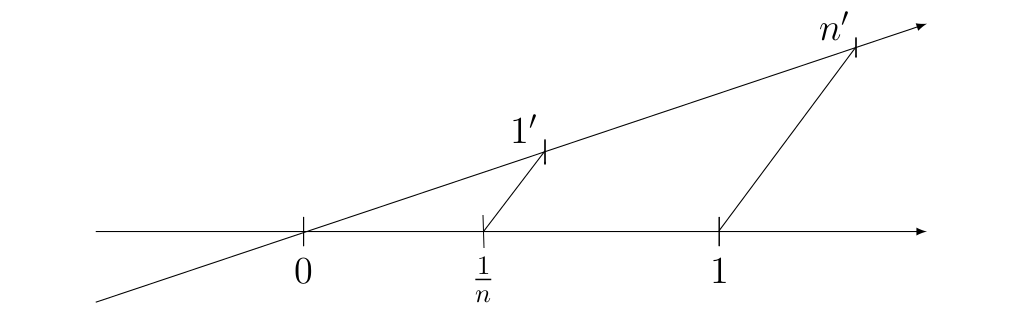
\includegraphics[width=0.8\linewidth]{falles.png}
        \end{figure}\\
        таким образом складывая $m$ раз $\frac{1}{n}$, получим любое рациональное число $\frac{m}{n}$.\\
        Построим бесконечную десятичную дробь, например $0,37152\dots$.\\
        Разобьем отрезок:
        \[\begin{tikzpicture} [scale=5.5]
        \draw[-latex] (-0.5,0) -- (1.5,0) ;
        \foreach \x in {0,0.2,0.4,0.6,0.8,1}
        \draw[shift={(\x,0)},color=black] (0pt,1pt) -- (0pt,-1pt);
        \foreach \x in {0,0.2,0.4,0.6,0.8,1}
        \draw[shift={(\x,0)},color=black] (0pt,1pt) -- (0pt,-1pt) node[below] 
        {$\x$};
        \end{tikzpicture}\]
        $0,37152\dots$ находится между $0.2$ и $0.4$, теперь разобьем этот отрезок:
        \[\begin{tikzpicture} [scale=28]
        \draw[-latex] (0.1,0) -- (0.5,0) ;
        \foreach \x in {0.2,0.24,0.28,0.32,0.36,0.4}
        \draw[shift={(\x,0)},color=black] (0pt,0.2pt) -- (0pt,0.2pt);
        \foreach \x in {0.2,0.24,0.28,0.32,0.36,0.4}
        \draw[shift={(\x,0)},color=black] (0pt,0.2pt) -- (0pt,-0.2pt) node[below] 
        {$\x$};
        \end{tikzpicture}\]
        $0,37152\dots$ находится между $0.36$ и $0.4$, теперь разобьем этот отрезок и т.д.
        Получаем последовательность вложенных отрезков, у которых длина стремится к нулю, значит у них есть единственная общая точка - наше число.\\
        Таким образом, прямая - множество бесконечных десятичных дробей, а значит на ней выполняеются (1)-(16).
        \subsection{Принципы полноты}
        %\subsubsection{Верхние и нижние грани множества}
        \begin{definition} \tab
            \begin{itemize}
                \item Элемент $a\in \R$ называется максимальным элементом множества $A$\\ $(\max A\subset \R), A\ne \emptyset$, если $\forall a^{\prime}\in A: a\geq a^{\prime}$ и $a\in A$.
                \item Элемент $a\in \R$ называется минимальным элементом множества $A$\\ $(\min A\subset \R), A\ne \emptyset$, если $\forall a^{\prime}\in A: a\leq a^{\prime}$ и $a\in A$.
            \end{itemize}
        \end{definition} \tab
        \begin{definition} \tab
            \begin{itemize}
                \item Элемент $m\in \R$ называется верхней гранью $A\subset \R, A\ne \emptyset$, если\\ $\forall a\in A: a\leq m$.
                \item Элемент $m\in \R$ называется нижней гранью $A\subset \R, A\ne \emptyset$, если\\ $\forall a\in A: a\geq m$.
            \end{itemize}
        \end{definition}
        \begin{definition} \tab
            \begin{itemize}
                \item Множество $A \subset \R, A\ne \emptyset$ называется ограниченным сверху, если у $A$ существует верхняя грань.
                \item Множество $A \subset \R, A\ne \emptyset$ называется ограниченным снизу, если у $A$ существует нижняя грань.
                \item Множество $A \subset \R$ называется ограниченным, если $A$ ограничено и сверху и снизу.
            \end{itemize}
        \end{definition}
        \begin{definition} \tab
            \begin{itemize}
                \item Пусть множество $A \subset \R$ ограничено сверху, $B$ - множество верхних граней $A$. Элемент $c=\min B$ называется точной верхней гранью $A$ и обозначается $\sup A$.
                \item Пусть множество $A \subset \R$ ограничено снизу, $B$ - множество нижних граней $A$. Элемент $c=\max B$ называется точной нижней гранью $A$ и обозначается $\inf A$.
            \end{itemize}
        \end{definition}
        %\subsubsection{Принцип полноты Вейерштрасса}
        \begin{theorem} (Принцип полноты Вейерштрасса) \\
            Для каждого ограниченого сверху или снизу множества $A$ существует $\sup A$ или $\inf A$ соответственно.
        \end{theorem}
        \begin{proof}
            Докажем для верхней грани (аналогично для нижней)\\
            $A$ - ограничено сверху, $B$ - множество верхних граней. Значит $\forall a\in A$ и \\$\forall b\in B: a\leq b \Rightarrow$ по аксиоме полноты $\exists\ c\in \R: a\leq c\leq b \Rightarrow c=\sup A$.
        \end{proof}
        \begin{lemma} (Свойство точной грани)\\
            Если у множества $A\subset \R$ существует $M=\sup{A}$ или $m=\inf{A}$, то $\forall \epsilon>0\ \exists\ a\in A: a\in (M-\epsilon,M)$ или $a\in (m,m+\epsilon)$ соответственно.
        \end{lemma}
        \begin{proof}
            Докажем для верхней грани. $M=\sup{A}\Rightarrow \forall a\in A: a\leq M$. Поскольку $M$ - минимальная из верхних граней, то $\forall \epsilon>0: \widetilde{M}=M-\epsilon$ - не является верхней гранью. Тогда $\exists\ a\in A: a>\widetilde{M} \Rightarrow a\in (M-\epsilon,M)$.
        \end{proof} 
        \begin{definition}
            $\forall a,b\in \R: a<b$ рассмотрим следующие множетсва:
            \begin{itemize}
                \item $[a,b] := \{x\in \R: a\leq x\leq b\}$ - отрезок
                \item $(a,b) := \{x\in \R: a<x<b\}$ - интервал
                \item $[a,b) := \{x\in \R: a\leq x<b\}$ - полуинтервал
                \item $(a,b] := \{x\in \R: a<x\leq b\}$ - полуинтервал
            \end{itemize}
            Такие множества называют промежутками.
        \end{definition} 
        \begin{definition}
            $\forall a\in \R$ функция
            \[|a|=
                \begin{cases}
                    \tab[12pt]a, \tab[5pt] a\geq 0,\\
                    -a, \tab[5pt] a<0.
                \end{cases}\]
            называется модулем.
        \end{definition}
        \begin{definition}
            Для любого промежутка с концами $a,b\in \R$ длиной называется число $|b-a|$.
        \end{definition}
        \begin{definition}
            Рассмотрим последовательность $\{[a_n,b_n]\}_{n=1}^{\infty}$. Говорят, что\\ $|b_n-a_n|\to 0$ при $n\to \infty$, если $\forall \epsilon >0\tab[5pt]\exists N\in \N: \forall n>N$ выполнено $|b_n-a_n|<\epsilon$.
        \end{definition}
        %\subsubsection{Принцип вложенных отрезков (принцип полноты Кантора)}
        \begin{theorem} (Принцип вложенных отрезков, принцип полноты Кантора) \\
            Пусть последовательность $\{[a_n,b_n]\}_{n=1}^{\infty}$ такова, что $\forall n: [a_{n+1},b_{n+1}]\subset [a_n,b_n]$. Тогда $\exists\ c\in \R: c\in [a_n,b_n], \forall n$. Если $|b_n-a_n|\to 0$ то $c$ - единственная.
        \end{theorem} 
        \begin{proof}
            $\forall n,m\in \N: a_n\leq b_m$, т.к
            \begin{itemize}
                \item если $n<m$, то $a_n\leq a_m\leq b_m$.
                \item если $n>m$, то $a_n\leq b_n\leq b_m$.
            \end{itemize}
            Значит для $\forall m,n\in \N: $
            Рассмотрим множества $A=\{a_n\}$ и $B=\{b_n\}$. По аксиоме полноты $\exists\ c\in \R: a_n\leq c\leq b_m,\ \forall n,m \Rightarrow a_n\leq c\leq b_n,\ \forall n$.\\
            Пусть $|b_n-a_n|\to 0$, предположим, что $\exists\ c_1$ и $c_2: c_1\ne c_2$ - различные общие точки, значит $|c_2-c_1|>0$. Получаем, что $0<|c_2-c_1|<|b_n-a_n|,\ \forall n$, значит $|c_2-c_1|\to 0$ получаем противоречие.
        \end{proof} 
        \subsection{Отношение эквивалентности. Равномощные множества}
        \begin{definition}
            Отношение $\sim$ называется отношением эквивалентности, если оно удовлетворяет:
            \begin{enumerate}
                \item $x\sim x$ (Рефлексивность)
                \item $x\sim y \Rightarrow y\sim x$ (Симметричность)
                \item $x\sim y$ и $y\sim z\Rightarrow x\sim z$ (Транзитивность)
            \end{enumerate}
        \end{definition} 
        \begin{definition}
            Множества называются равномощными, если между ними существует биекция.
        \end{definition}
        \begin{theorem}
            Равномощность множеств является отношением эквивалентности.
        \end{theorem}
        \begin{proof} Пусть $A,B,C$ - множества, $\phi:A\to B, \psi:B\to C$ - биекции.
            \begin{enumerate}
                \item Рефлексивность очевидна, поскольку у любого множества существует биекция в себя.
                \item Для любой биекции $\phi:A\to B$ существует $\phi^{-1}:B\to A$.
                \item $\phi:A\to B,\ \psi:B\to C$, то $\psi \circ \phi: A\to C$.
            \end{enumerate}
        \end{proof} 
        \begin{comm}
            Если $A$ равномощно $B$ то иногда пишут $A\sim B$ или $|A|=|B|$.
        \end{comm} 
        \begin{theorem}
            Конечные множества равномощны $\Leftrightarrow$ они содержат одинаковое количество элементов.
        \end{theorem}
        \begin{proof}\tab
            \begin{itemize}
                \item[$(\Leftarrow)$] Пусть $\phi:A\to \{1,\dots, n\}, \ \psi:B\to \{1,\dots, n\}\\
                \Rightarrow \exists \ \psi^{-1}:\{1,\dots, n\}\to B$. Тогда $\phi \circ \psi^{-1}:A\to B$ - искомая биекция.
                \item[$(\Rightarrow)$] Пусть $\phi:A\to B$ - биекция, если $A=\emptyset$, то $B=\emptyset$. Индукция по количеству элементов. База: пусть $A=\{a\}$, тогда $\exists ! \ b\in B: \phi(a)=b$. Пусть утверждение верно для случая когда $A$ - это $n$-элементное множество. Теперь если $A$ - это $n+1$-элементное, то $\exists \ \phi:A\to \{1,2,...,n+1\}$ - биекция. Значит $\exists ! \ a\in A$, что $\phi(a)=n+1$. Тогда $A\setminus\{a\}$ - $n$-элементное и $\exists ! \ b\in B: b=\phi(a) \Rightarrow B\setminus\{b\}$ - $n$-элементное $\Rightarrow  B$ - $n+1$-элементное.
            \end{itemize}
        \end{proof}
        \begin{definition}
            Множества, равномощные $\N$ называются счетными.
        \end{definition} 
        \begin{definition}
            Множество называется не более чем счетным, если оно конечно или счетно.
        \end{definition}
        \begin{theorem}
            Объединение не более чем счетного числа счетных множеств счетно.
        \end{theorem}
        \begin{proof}
            Предъявим проход по элементам, который задает биекцию:
            \begin{center}
                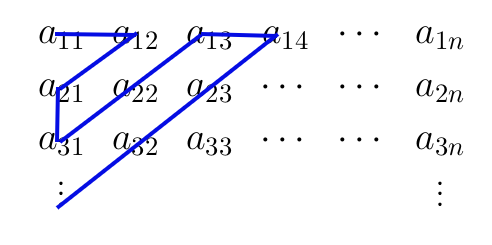
\includegraphics[width=0.4\linewidth]{prohod.png}
            \end{center}
        \end{proof}
        \begin{consequense}
            Объединение не более чем счетного числа не более чем счетных множеств не более чем счетно.
        \end{consequense} 
        \begin{examples}\tab
            \begin{enumerate}
                \item Множество целых чисел $\Z$ счетно.
                \item Множество рациональных чисел $\Q$ счетно.
                \item Множество многочленов с рациональными коэффициентами счетно.
                \item Множество алгебраических чисел (чисел которые являются корнями многочлена с рациональными коэффициентами) счетно.
            \end{enumerate}
        \end{examples}
        \subsection{Теорема Кантора и аксиома выбора}
        % \begin{theorem} (Теорема Кантора)\\
        %    Множество бесконечных последовательностей, состоящих из нулей и единиц несчетно.
        % \end{theorem} 
        % \begin{proof}
        %    Предположим, что оно счетно. Тогда все последовательности нулей и единиц можно перенумеровать. Составим бесконечную вниз таблицу, строками которой будут наши последовательности:\\
        %    \tab[6cm]$a_1=\underline{a_{11}}\ a_{12}\ a_{13}\ a_{14}\ \dots$\\
        %    \tab[6cm]$a_2=a_{21}\ \underline{a_{22}}\ a_{23}\ a_{24}\ \dots$\\
        %    \tab[6cm]$a_3=a_{31}\ a_{32}\ \underline{a_{33}}\ a_{34}\ \dots$\\
        %    \tab[6cm]$a_4=a_{41}\ a_{42}\ a_{43}\ \underline{a_{44}}\ \dots$\\
        %    \tab[6cm]\vdots\\
        %    $a_{ij}$ - $j$-й член $i$-й последовательности. Рассмотрим последовательность $b$ у которой $b_i=1-a_{ii}$. Такая последовательность отличается от каждой $i$-й последовательности на $i$-й позицции, значит она не была посчитана, получаем противоречие.
        % \end{proof}
        \begin{theorem} (Теорема Кантора)\\
            Интервал $(0,1)$ несчетен.
        \end{theorem}
        \begin{proof}\footnote{Может немного отличаться от доказательства на лекциях}
            Докажем от противного. Предположим, что у нас получилось перечислить все элементы интервала $(0,1)$ 
            \[x_1=0,\ a_{11}\ a_{12}\ a_{13}\ \dots\]
            \[x_2=0,\ a_{21}\ a_{22}\ a_{23}\ \dots\]
            \[x_3=0,\ a_{31}\ a_{32}\ a_{33}\ \dots\]
            \[\vdots\]
            \newpage
            Теперь построим такую последовательность $b$, задающую число, которого нет в списке. Определим последовательность так: $b_0 = 0$ и на $i$-й позиции $b_i$ отличается от $a_{ii}$, например зададим ее так:
            \[b_i=
            \begin{cases}
                1,\ \text{если},\ a_{ii}\ne 1,\\
                2,\ \text{если},\ a_{ii}=1.
            \end{cases}\]
            Таким образом, построенное число $x = 0,\ b_1\ b_2\ b_3\ \dots$ отличается от каждого из $x_1,x_2,x_3\dots$ на $i$ позиции $\Rightarrow$ оно не было пересчитано, получаем противоречие.
        \end{proof} 
        \begin{consequense}
            Действительных чисел несчетно.
        \end{consequense} 
        \begin{proof}\footnote{Не было на лекциях}
            Достаточно показать, что $\R \sim (0,1)$. Например функция\\
            $f:(0,1)\to \R$, такая что $f(x)=\frac{2x-1}{4x-4x^2}$ задает нужную биекцию.
        \end{proof} 
        \begin{definition}
            Действительные числа не являющиеся алгебраическими называются трансцендентными.
        \end{definition} 
        \begin{definition}
            Множества равномощные интервалу $(0,1)$ называются множествами мощности континуума.
        \end{definition} 
        \begin{theorem}
            У любого множетсва мощность множества всех подмножеств строго больше чем мощность самого множества.
        \end{theorem}
        \begin{proof}
            Без доказательства.
        \end{proof} 
        \begin{definition}
            Для множеств $A$ и $B$ обозначим $|A|\leq |B|$, если $\exists \ B^{\prime} \subset B$ такое, что $A\sim B^{\prime}$.
        \end{definition} 
        \begin{theorem}
            Сравнение мощностей множеств $|A|\leq |B|$ является отношением порядка.
            \begin{enumerate}
                \item $\forall A,B: |A|\leq |B|$ или $|B|\leq |A|$ 
                \item $|A|\leq |B|$ и $|B|\leq |A| \Rightarrow |A|=|B|$\ (Теорема Кантора-Бернштейна)
                \item $|A|\leq |B|$ и $|B|\leq |C| \Rightarrow |A|\leq |C|$
            \end{enumerate}
        \end{theorem}
        \begin{proof}
            Без доказательства.
        \end{proof}
        \begin{axiom}(Аксиома выбора)\\
            Если существует семейство непустых множеств, то из каждого множества можно выбрать по одному элементу и составить из них другое множество.
        \end{axiom}
        \begin{statement}
            Множество $2^{\N}$ всех подмножеств $\N$ равномощно интервалу (0,1) (множеству $\{0,1\}^{\N}$ бесконечных последовательностей нулей и единиц).
        \end{statement}
        \begin{proof}\footnote{Может отличаться от доказательства на лекциях}
            Каждому $A\subset \N$ ставим в соответствие характеристическую последовательность, которая принимает значения: единицу, если элемент лежит в подмножестве и ноль иначе $\Rightarrow 2^{\N}\sim \{0,1\}^{\N}$. Поскольку каждое число из интервала $(0,1)$ представляется как последовательность цифр $0,\ a_1,\ a_2,\ a_3,\ \dots$ и каждую цифру можно представить в двоичной системе исчисления, то можно сделать вывод, что $2^{\N}\sim (0,1)$.
        \end{proof}
        \begin{theorem}
            У любого бесконечного множества существует счетное подмножество.
        \end{theorem} 
        \begin{proof}
            Выбираем элемент и сразу присваиваем ему номер. Продолжая это действие, построим счетное множество.
        \end{proof}
        \begin{theorem}
            Пусть $A$ - бесконечное, $B$ - не более чем счетное $\Rightarrow A\sim A\cup B$
        \end{theorem} 
        \begin{proof}
            Выделим из $A$ счетное подмножество $A^{\prime}$. Тогда $A\sim (A\setminus A^{\prime})\cup A^{\prime}$, поскольку объединение не более чем счётного числа не более чем счётных множеств не более чем счётно, то  $(A\setminus A^{\prime})\cup A^{\prime} \sim (A\setminus A^{\prime})\cup(A^{\prime}\cup B) \sim(A\cup B)$.
        \end{proof}
    \newpage
    \section{Топология вещественной прямой}
    \subsection{Окрестность точки. Классификация точек относительно подмножеств действительных чисел}
        \begin{definition}
            $\forall x\in \R,\ \forall \epsilon>0: B_{\epsilon}(x)=(x-\epsilon, x+\epsilon)$. Множество $B_{\epsilon}(x)$ называется $\epsilon$-окрестностью точки $x$.
        \end{definition}
        \begin{definition}
            $\forall x\in \R,\ \forall \epsilon>0: \mathring{B}_{\epsilon}(x)=(x-\epsilon,x)\cup(x,x+\epsilon)$.  Множество $\mathring{B}_{\epsilon}(x)$ называется проколотой $\epsilon$-окрестностью точки $x$.
        \end{definition} 
        \begin{definition}
            Точка $x\in A\subset \R$ называется внутренней точкой множества $A$, если $\exists \ B_{\epsilon}(x)\subset A$. Множество всех внутренних точек $x\in A$ называется внутренностью множетсва $A$.
        \end{definition} 
        \begin{definition}
            Точка $x\in \R\setminus A$ называется внешней точкой для множества $A\subset \R$, если $x$ - внутренняя точка для $\R\setminus A$. Множество всех внешних точек $x\in A$ называется внешностью множетсва $A$.
        \end{definition}
        \begin{definition}
            Точка называется граничной для множества $A\subset \R$, если она не является ни внешней ни внутренней для $A$ (в любой ее окрестности есть как точки из $A$ так точки из $\R \setminus A$). Множество всех граничных точек называется границей множества $A$ и обозначается $\partial A$.
        \end{definition}
        \begin{definition}
            Точка $x\in \R$ называется предельной точкой множества $A\subset \R$, если в любой проколотой окрестности точки $x$ бесконечно много точек $A$, т.е\\
            $\forall\ \epsilon >0: A\cap \mathring{B}_{\epsilon}(x)\ne\emptyset$. Множество всех предельных точек $A$ обозначается $A^{\prime}$
        \end{definition} 
        \begin{definition}
            Точка $x\in A$ называется изолированной точкой $A\subset \R$, если $\exists \ \epsilon>0: A\cap \mathring{B}_{\epsilon}(x)=\emptyset$.
        \end{definition} 
        \begin{definition}
            Точка $x\in \R$ называется точкой прикосновения $A\subset \R$, если $\forall \ \epsilon>0: A\cap {B}_{\epsilon}(x)\ne\emptyset$.
        \end{definition} 
        \begin{statement}
            Точки прикосновения множества $A$ являются либо внутренними, либо граничными.
        \end{statement}
        \begin{proof}
            Точка прикосновения не может являться внешней точкой, поскольку в этом случае $\exists\ \epsilon>0: B_{\epsilon}(x)\in \R\setminus A$, что противоречит с условием $\forall \ \epsilon>0: A\cap {B}_{\epsilon}(x)\ne\emptyset$
            $\Rightarrow$ она либо внутренняя либо граничная.
        \end{proof}
        \begin{statement}
            Точки прикосновения являются либо предельными, либо изолированными.
        \end{statement}  
        \begin{proof}
            Если $\forall \ \epsilon>0: A\cap \mathring{B}_{\epsilon}(x)\ne\emptyset$, то $x$ - предельная. Если $\exists\ \epsilon > 0: A\cap\mathring{B}_{\epsilon}(x)=\emptyset$, но по определению $\forall \ \epsilon>0: A\cap B_{\epsilon}(x)\ne\emptyset\\
            \Rightarrow x\in A \Rightarrow x$ - изолированная.
        \end{proof} 
        \begin{definition} (Множество Кантора)\\
            Разбиваем отрезок $[0,1]$ на три части и выбрасываем середину, затем каждый из получившихся отрезков разбиваем на три части и выбрасываем середину, и т.д.
            \begin{itemize}
                \item Суммарная длина всех выброшенных интервалов равна $1$.
                \item Концов отрезков счетное множество.
                \item Общее количество точек имеет мощность континуума.
            \end{itemize}
    \subsection{Открытые и замкнутые множества}
        \end{definition} 
        \begin{definition}
            Множество называется открытым, если все его точки - внутренние.
        \end{definition}
        \begin{example} 
            Любой интервал - открытое множество 
        \end{example}
        \begin{definition}
            Множество $A\subset \R$ называется замкнутым, если его дополнение $\R\setminus A$ открыто.
        \end{definition} 
        \begin{example}
            Отрезок - замкнутое множество.
        \end{example}
        \begin{comm}
            По определению считаем, что $\emptyset$ и $\R$ и открыты и замкнуты одновременно.
        \end{comm} 
        \begin{theorem} (Критерии замкнутости множества)\\
            Следующие условия эквивалентны:
            \begin{itemize}
                \item[(0)] $A\subset \R$ - замкнуто. 
                \item[(1)] $\partial A\subset A$,
                \item[(2)] Все точки прикосновения содержатся в $A$,
                \item[(3)] $A^{\prime}\subset A$.
            \end{itemize}
            \begin{proof}
                Докажем по цепочке $(0)\Rightarrow (1)\Rightarrow (2)\Rightarrow (3)\Rightarrow (0)$.
                \begin{enumerate}
                    \item $(0)\Rightarrow (1):A$ - замкнуто $\Rightarrow \R\setminus A$ - открыто $\Rightarrow \partial A \not\subset\R\setminus A \Rightarrow \partial A\subset A$.
                    \item $(1)\Rightarrow (2):$ Все точки прикосновения являются граничными или внутренними. Поскольку $\partial A\subset A$ то все точки прикосновения содержатся в $A$.
                    \item $(2)\Rightarrow (3):$ Если $x$ - предельная, то $x\in A$ или $x$ - точка прикосновения. Поскольку все точки прикосновения содержатся в $A$, то и все предельные точки содержатся в $A$.
                    \item $(3)\Rightarrow (0): A^{\prime}\subset A\Rightarrow \forall x\in \R\setminus A: x\not\in A^{\prime}\Rightarrow \forall x\in\R\setminus A\ \exists\ \mathring{B}_{\epsilon}: \mathring{B}_{\epsilon}(x)\cap A=\emptyset\\
                    \Rightarrow B_{\epsilon}(x)\cap A=\emptyset\ (\text{т.к}\ x\not\in A) \Rightarrow x$ - внешняя точка $A,\ B_{\epsilon}(x)\subset\R\setminus A\\
                    \Rightarrow \R\setminus A$ - открыто $\Rightarrow A$ - замкнуто. 
                \end{enumerate}
            \end{proof}
        \end{theorem}
        \begin{theorem}
            Пусть $A$ - множество индексов. Пусть $\{U_{\alpha}\}_{\alpha\in A}$ - открытые,\\
            $\{X_{\alpha}\}_{\alpha\in A}$ - замкнутые. Тогда:
            \begin{enumerate}
                \item $\bigcup\limits_{\alpha} U_{\alpha}$ - открыто (объединение открытых множетсв - открыто).
                \item $\bigcap\limits_{i=1}^n U_{\alpha_i}$ - открыто (конечное пересечение открытых множеств - открыто).
                \item $\bigcup\limits_{i=1}^n X_{\alpha_i}$ - замкнуто (конечное объединение замкнутых множеств - замкнуто).
                \item $\bigcap\limits_{\alpha} X_{\alpha}$ - замкнуто (пересечение замкнутых множеств - замкнуто).
            \end{enumerate}
        \end{theorem} 
        \begin{proof} \tab
            \begin{enumerate}
                \item Пусть $u\in \bigcup\limits_{\alpha} U_{\alpha} \Rightarrow \exists\ \alpha_0: u\in U_{\alpha_0}\Rightarrow \exists\ B(u)\in U_{\alpha_0}\Rightarrow B(u)\in \bigcup\limits_{\alpha} U_{\alpha}\\
                \Rightarrow \bigcup\limits_{\alpha} U_{\alpha}$ - открыто.
                \item Пусть $u\in \bigcap\limits_{i=1}^n U_{\alpha_i} \Rightarrow \forall i\in \{1,\dots, n\}\ \exists\ \epsilon_i: B_{\epsilon_i}(u)\in U_{\alpha_i}\Rightarrow \exists\ \epsilon_0 = \min\{\epsilon_{i}\}\\
                \Rightarrow B_{\epsilon_{0}}\subset U_{\alpha_i}\ \forall i \Rightarrow B_{\epsilon_{0}}\subset \bigcap\limits_{i=1}^n U_{\alpha_i} \Rightarrow \bigcap\limits_{i=1}^n U_{\alpha_i}$ - открыто.
                \item Поскольку $\bigcap\limits_{\alpha}(A\setminus A_{\alpha}) = A\setminus (\bigcup\limits_{\alpha}A_{\alpha})$ (доказано ранее), то $\R \setminus \bigcup\limits_{i=1}^n X_{\alpha_i}=\\
                =\bigcap\limits_{i=1}^n(\R \setminus X_{\alpha_i})$. Так как $X_{\alpha_i}$ - замкнуто, то $\R \setminus X_{\alpha_i}$ - открыто. Тогда по пункту 2 получаем: $\bigcap\limits_{i=1}^n(\R \setminus X_{\alpha_i})$ - открыто $\Rightarrow \R \setminus \bigcup\limits_{i=1}^n X_{\alpha_i}$ - открыто \\
                $\Rightarrow \bigcup\limits_{i=1}^n X_{\alpha_i}$ - замкнуто.
                \item Поскольку $\bigcup\limits_{\alpha}(A\setminus A_{\alpha}) = A\setminus (\bigcap\limits_{\alpha}A_{\alpha})$ (доказано ранее), то $\R \setminus \bigcap\limits_{\alpha} X_{\alpha}=\\
                =\bigcup\limits_{\alpha}(\R \setminus X_{\alpha})$. Так как $X_{\alpha}$ - замкнуто, то $\R \setminus X_{\alpha}$ - открыто. Тогда по пункту 1 получаем: $\bigcup\limits_{\alpha}(\R \setminus X_{\alpha})$ - открыто $\Rightarrow \R \setminus \bigcap\limits_{\alpha} X_{\alpha}$ - открыто $\Rightarrow \bigcap\limits_{\alpha}X_{\alpha}$ - замкнуто.
            \end{enumerate}
        \end{proof} 
        \begin{examples} \tab
            \begin{enumerate}
                \item $\bigcap\limits_{n=1}^{\infty}(-\frac{1}{n}, 1+\frac{1}{n})=[0,1]$.
                \item $\bigcup\limits_{n=1}^{\infty}[\frac{1}{n}, 1-\frac{1}{n}]=(0,1)$.
            \end{enumerate}
        \end{examples}
        \begin{theorem}
            Если $A$ - ограничено сверху или снизу и замкнуто, то существует $\max{A}$ или $\min{A}$ соответственно.
        \end{theorem} 
        \begin{proof}
            Докажем для ограниченного сверху. По принципу полноты Вейерштрасса $\exists\ \alpha=\sup{A}$. По свойству точной верхней грани:\\
            $\forall\epsilon>0\ \exists\ a\in (\alpha-\epsilon, \alpha]\Rightarrow \alpha$ - точка прикосновения $\Rightarrow \alpha \in A\Rightarrow \alpha=\max{A}$.
        \end{proof}
    \subsection{Компакты}
        \begin{definition}
            Говорят, что семейство $\{A\}_{\alpha}$ является покрытием множества $B$, если $B\subset \bigcup\limits_{\alpha}A_{\alpha}$
        \end{definition} 
        \begin{definition}
            Рассмотрим $X\subset \R$. Если для любого покрытия $X$ открытыми множествами $\{A\}_{\alpha}$ существует $\{\alpha_i\}_{i=1}^n$ - конечное подпокрытие такое, что \\
            $X\subset \bigcup\limits_{i=1}^n A_{\alpha_i}$, то $X$ называется компактным множеством или компактом.
        \end{definition} 
        \begin{theorem}
            Любой отрезок является компактом.
        \end{theorem} 
        \begin{proof}
            Пусть $[a,b]\subset \bigcup\limits_{\alpha}A_{\alpha},\ A_{\alpha}$ - открытые и нельзя выделить конечное подпокрытие. Тогда $[a,b]=[a_1,b_1]$ делим отрезок пополам и выбираем половину $[a_2,b_2]$, у которой нельзя выделить конечное подпокрытие и т.д. Получаем систему вложенных отрезков $\{[a_n,b_n]\}_{n=1}^{\infty}$, у которых нельзя выделить конечное подпокрытие и длина стремится к нулю $\Rightarrow \exists!\ c\in [a_n,b_n]\ \forall n \Rightarrow \exists\ \alpha_0: c\in A_{\alpha_0}$. Поскольку $A_{\alpha_0}$ - открыто, то $\exists\ B_{\epsilon}(c)\subset A_{\alpha_0}$ $\Rightarrow \exists\ n_{\alpha_0}: [a_{n_{\alpha_0}},b_{n_{\alpha_0}}]\subset A_{\alpha_0}$ получаем противоречие.
        \end{proof} 
        \begin{theorem} (Лемма Гейне-Бореля)\footnote{На самом деле, утверждение верно и для $\R^n$}\\
            $A$ - компакт в $\R$ $\Leftrightarrow A$ - замкнуто и ограничено.
        \end{theorem} 
        \begin{proof}
            Без доказательства.
        \end{proof}
    \subsection{Теорема Больцано-Вейерштрасса}
        \begin{theorem} (Больцано-Вейерштрасса)\\
            Если $A\subset \R$ - ограниченное и бесконечное множетсво, то в нем есть хотя бы одна предельная точка (т.е. $A^{\prime}\ne \emptyset$).
        \end{theorem} 
        \begin{proof}
            т.к $A$ - ограничено, то $\exists\ \sup{A}=b,\ \inf{A}=a\\ \Rightarrow A\subset [a_1,b_1] = [a,b]$. Поделим отрезок $[a_1,b_1]$ пополам и возьмем половину $[a_2,b_2]$ в которой бесконечно много элементов из множества $A$ и т.д. Получаем систему вложенных отрезков $\{[a_n,b_n]\}_{n=1}^{\infty}$, у которых длина стремится к нулю $\Rightarrow \exists!\ c\in [a_n,b_n]\ \forall n\Rightarrow \forall \epsilon>0\ \exists\ n_{\epsilon}: [a_{n_{\epsilon}},b_{n_{\epsilon}}]\subset B_{\epsilon}(c) \Rightarrow$ существует бесконечно много элементов в $\mathring{B}_{\epsilon}(c)\Rightarrow c\in A^{\prime}$.
        \end{proof}
    \newpage
    \section{Числовые последовательности}
    \subsection{Предел последовательности}
        \begin{definition}
            Отображение $\{a_n\}: \N\to \R$ называется последовательностью.
        \end{definition} 
        \begin{comm}
            Далее, в обозначении последовательности будем опускать скобки и писать $a_n$.
        \end{comm} 
        \begin{definition}
            Говорят, что $a_n$ ограничена сверху (снизу), если ее образ ограничен сверху (снизу).
        \end{definition} 
        \begin{definition}
            Пусть последовательность номеров $n_k$ - образ $\phi: \N\to \N$ и $\forall k: n_{k+1}>n_k$. Тогда для любой последовательности $a_n$ последовательность $a_{n_k}$ называется подпоследовательностью $a_n$.
        \end{definition} 
        \begin{definition}
            Рассмотрим последовательность $a_n$. Если $\exists \ a\in \R$, такое что 
            \[\forall \epsilon>0\ \exists\ N_{\epsilon}\in \N: \forall n>N_{\epsilon}: |a_n-a|<\epsilon\]
            то говорят, что последовательность $a_n$ сходится, а число $a$ называется пределом последовательности $a_n$ и обозначается
            \[\lim\limits_{n\to \infty} a_n=a\]
        \end{definition}
        \begin{theorem}
            Если $a_n$ сходится, то ее предел единственный.
        \end{theorem} 
        \begin{proof}
            Пусть $\exists\ a,b\in \R: a\ne b$ - два предела последовательности $a_n$. Тогда
            \[\exists\ N_1: \forall n>N_1: |a_n-a|<\frac{|a-b|}{3}\  \ \text{и}\ \ \exists\ N_2: \forall n>N_2: |a_n-b|<\frac{|a-b|}{3}\]
            Тогда $\forall n>N = \max{(N_1, N_2)}$ получаем, что $a_n\in B_{\frac{|a-b|}{3}}(a)$ и $a_n\in B_{\frac{|a-b|}{3}}(b)$, но $B_{\frac{|a-b|}{3}}(a)\cap B_{\frac{|a-b|}{3}}(b)= \emptyset \Rightarrow$ получаем противоречие.
        \end{proof} 
        \begin{theorem}
            Пусть $\exists\ \lims a_n=a$, тогда $\forall a_{n_k}\ \exists\ \lims a_{n_k}=a$.
        \end{theorem} 
        \begin{proof}
            $\forall \epsilon>0\ \exists\ N_{\epsilon}\ \forall n>N_{\epsilon}: |a_n-a|<\epsilon \Rightarrow \forall n_k>N_{\epsilon}:\\ |a_{n_k}-a|<\epsilon$
        \end{proof} 
        % \begin{comm}
        %     $\forall k\in \Z$ отображение $\Z \setminus \{..., k-1\} \to \R$ тоже будем называть последовательностью.
        % \end{comm} 
        \
        \begin{comm}\tab
            \begin{enumerate}
                \item Если $\exists \lims a_n=a$, то $\exists \lims a_{n+k}=a$.
                \item Если $\exists\ \lims a_n=a$ и $b_n$ отличается от $a_n$ конечным числом членов, то $\exists \lims b_n=a$.
            \end{enumerate}
        \end{comm} 
        \begin{theorem} (Теорема об отделимости)\\
            Пусть $\exists \lims a_n=a$ и $b\ne a$. Тогда $\exists\ \epsilon>0\ \exists\ N_{\epsilon}: B_{\epsilon}(b)\cap \{a_n\}_{n=N_{\epsilon}}^{\infty}=\emptyset$.
        \end{theorem} 
        \begin{proof}
            Предположим, что выполнено обратное: $\forall \epsilon>0\ \forall \ N_{\epsilon}:\\
            B_{\epsilon}(b)\cap \{a_n\}_{n=N_{\epsilon}}^{\infty}\ne \emptyset$. Возьмем $\epsilon = \frac{|b-a|}{3}$, сразу получаем противоречие.
        \end{proof} 
        \begin{comm}
            Теорема об отделимости равносильна следующему утверждению: $\exists\ \epsilon>0: \mathring{B_{\epsilon}}(b)\cap \{a_n\}_{n=1}^{\infty}=\emptyset$, причем если $b\notin \{a_n\}_{n=1}^{\infty}$, то $B_{\epsilon}(b)\cap\{a_n\}_{n=1}^{\infty}=\emptyset$.
        \end{comm} 
        \subsection{О-символика. Бесконечно малые и бесконечно большие последовательности}
        \begin{definition}
            Рассмотрим пару последовательностей $a_n$ и $b_n$. Если\\ $\exists\ \lims \frac{a_n}{b_n}=0$, то говорят, что последовательность $a_n$ - это о-малое от $b_n$, и обозначают $a_n=\om(b_n)$, при $n\to \infty$. 
        \end{definition} 
        \begin{definition}
            Если $\exists\ M>0: |\frac{a_n}{b_n}|\leq M\ \forall n$, то говорят, что последовательность $a_n$ - это O-большое от $b_n$, и обозначают $a_n=O(b_n)$, при $n\to \infty$.
        \end{definition} 
        \begin{examples}\tab
            \begin{enumerate}
                \item $\frac{\sin n}{n}\to 0 \Leftrightarrow \sin n = \om(n)$
                \item $\frac{\cos n}{n}\to 0 \Leftrightarrow \cos n = \om(n)$
                \item $\frac{\sqrt{n}+1}{n}\to 0 \Leftrightarrow \sqrt{n}+1 = \om(n)$
            \end{enumerate}
        \end{examples}
        \begin{comm}
            $O(1)$ - обозначение класса ограниченных последовательностей.
        \end{comm} 
        \begin{definition}
            Последовательность $a_n$ называется бесконечно малой, если 
            \[a_n=\om(1)\ (\Leftrightarrow \lim\limits_{n\to \infty}a_n=0)\]
        \end{definition} 
        \begin{definition}
            Последовательность $a_n$ называется бесконечно большой, если 
            \[\forall \epsilon>0\ \exists\ N_{\epsilon},\ \forall n>N_{\epsilon}: |a_n|>\epsilon\] 
            такие последовательности обозначаются $\lims a_n=\infty$ (это всего лишь обозначение, конечно у последовательности $a_n$ не существует предела)\\
            Если в определении $a_n>\epsilon$, то пишут $\lims a_n=+\infty$.\\
            Если в определении $a_n<-\epsilon$, то пишут $\lims a_n=-\infty$.
        \end{definition} 
        \begin{theorem} (Исчисление бесконечно малых)\\
            Пусть $a_n=\bar{\bar{o}}{(1)}, n\to \infty,\ b_n=\bar{\bar{o}}{(1)}, n\to \infty$ и $c_n=O(1)$. Тогда $\forall c\in \R$:
            \begin{enumerate}
                \item $ca_n=\bar{\bar{o}}{(1)}$
                \item $a_n+b_n=\bar{\bar{o}}{(1)}$
                \item $a_n b_n=\bar{\bar{o}}{(1)}$
                \item $c_n a_n=\bar{\bar{o}}{(1)}$
            \end{enumerate}
        \end{theorem} 
        \begin{proof}
            $\forall \epsilon>0\ \exists\ N_1,\ \forall n>N_1: |a_n|<\epsilon,\ \exists\ N_2,\ \forall n>N_2: |b_n|<\epsilon$.\\Возьмем $n>\max\{N_1,N_2\}$. Также по определению $\exists\ M>0: |c_n|<M$. Тогда:
            \begin{enumerate}
                \item $|c a_n|=|c|\ |a_n|<|c|\epsilon$. Поскольку $\epsilon$ принимает любое вещественное положительное значение, то величина $|c|\epsilon$ - тоже $\Rightarrow c a_n=\bar{\bar{o}}{(1)}$.
                \item $|a_n+b_n|\leq|a_n|+|b_n|<\epsilon+\epsilon=2\epsilon$. Поскольку $\epsilon$ принимает любое вещественное положительное значение, то величина $2\epsilon$ - тоже $\Rightarrow a_n+b_n=\bar{\bar{o}}{(1)}$.
                \item $|a_n b_n| = |a_n|\ |b_n|<\epsilon\cdot\epsilon=\epsilon^2$. Поскольку $\epsilon$ принимает любое вещественное положительное значение, то величина $\epsilon^2$ - тоже $\Rightarrow a_n b_n=\bar{\bar{o}}{(1)}$.
                \item $|c_n a_n|=|c_n|\ |a_n|<M\epsilon$. Поскольку $\epsilon$ принимает любое вещественное положительное значение, то величина $M\epsilon$ - тоже $\Rightarrow c_n a_n =\bar{\bar{o}}{(1)}$.
            \end{enumerate}
        \end{proof} 
        \begin{theorem}
            Пусть $a_n$ - бесконечно большая и $a_n\ne 0$, тогда $\frac{1}{a_n}$ - бесконечно малая.
        \end{theorem} 
        \begin{proof}
            $\forall \epsilon>0\ \exists\ N_{\epsilon},\ \forall n>N_{\epsilon}: |a_n|>\epsilon \Rightarrow \frac{1}{|a_n|}<\frac{1}{\epsilon} \Rightarrow \frac{1}{a_n}=\bar{\bar{o}}{(1)}$
        \end{proof} 
        \begin{lemma}
            $\lim\limits_{n\to \infty}a_n=a \Leftrightarrow a_n-a=\om(1)$ т.е $a_n=a+\bar{\bar{o}}{(1)}$
        \end{lemma} 
        \begin{proof}
            Из определения предела для $a_n$ получаем: $|a_n-a|<\epsilon$, а это и означает что $a_n-a=\bar{\bar{o}}{(1)}$.
        \end{proof} 
        \newpage
    \subsection{Арифметические свойства сходящихся последовательностей}
        \begin{theorem}
            Пусть $\exists \lim\limits_{n\to\infty} a_n=a,\ \exists \lim\limits_{n\to\infty} b_n=b$, тогда
            \begin{enumerate}
                \item $\exists \lim\limits_{n\to\infty} (a_n+b_n) = a+b$
                \item $\exists \lim\limits_{n\to\infty} (ca_n) = ca$
                \item $\exists \lim\limits_{n\to\infty} (a_n b_n) = ab$
                \item Если дополнительно $\forall n: b_n\ne 0$ и $b\ne 0$, то $\exists \lim\limits_{n\to\infty} (\frac{a_n}{b_n})=\frac{a}{b}$
            \end{enumerate}
        \end{theorem} 
        \begin{proof}
            Пользуясь тем, что $a_n=a+\bar{\bar{o}}{(1)},\ b_n=b+\bar{\bar{o}}{(1)}$ и исчислением бесконечно малых, получаем:
            \begin{enumerate}
                \item $a_n+b_n=a+\om(1)+b+\om(1)=a+b+\om(1)$.
                \item $ca_n=c(a+\om(1))=ca+c\om(1)=ca+\bar{\bar{o}}{(1)}$.
                \item $a_n b_n=(a+\om(1))(b+\om(1))=ab+a \bar{\bar{o}}{(1)}+b \bar{\bar{o}}{(1)}+\bar{\bar{o}}{(1)}\bar{\bar{o}}{(1)}=ab+\bar{\bar{o}}{(1)}$.
                \item $\cfrac{a_n}{b_n}-\cfrac{a}{b}=\cfrac{a_n b-ab_n}{bb_n}=\cfrac{b(a+\bar{\bar{o}}{(1)})-a(b+\bar{\bar{o}}{(1)})}{b(b+\bar{\bar{o}}{(1)})}=\cfrac{ab-ab+b \bar{\bar{o}}{(1)}-a \bar{\bar{o}}{(1)}}{b^2+b \bar{\bar{o}}{(1)}}=\\=\cfrac{1}{b^2+\bar{\bar{o}}{(1)}}\ \bar{\bar{o}}{(1)}=O(1) \bar{\bar{o}}{(1)}=\bar{\bar{o}}{(1)}$.
            \end{enumerate}
        \end{proof}
        %\begin{comm}
        %    т.к $b\ne 0,\ b_n\ne 0\ \forall n$, то 0 отделен от $b_n$, т.е $\exists\ \epsilon>0:\\
        %    B_{\epsilon}(0)\cap b_n=\emptyset \Rightarrow |b_n|>\epsilon \Rightarrow \frac{1}{|b_n|}<\frac{1}{\epsilon}$.
        %\end{comm}
        \begin{theorem}
            Пусть $\exists\ \lim\limits_{n\to \infty} a_n=a$ и $a_n\geq 0,\ \forall n$. Тогда $a\geq 0$.
        \end{theorem} 
        \begin{proof}
            Пусть $a<0$, тогда $\exists\ N,\ \forall n>N: |a-a_n|<\frac{|a|}{3} \Rightarrow$ начиная с $N$ все члены $a_n$ отрицательные $\Rightarrow$ получаем противоречие.
        \end{proof} 
        %   \begin{comm}
        %       Если $a_n>0,\ a\geq 0$, то $\frac{1}{n}\to 0$
        %   \end{comm}
        \begin{consequense}
            Пусть $\exists \lims a_n =a,\ \exists \lims b_n=b$ и пусть $\forall n: a_n\geq b_n$. Тогда $a\geq b$.
        \end{consequense}  
        \begin{proof}
            Рассмотрим последовательность $a_n-b_n\geq 0$.\\ $a_n-b_n\to a-b\geq 0$.
        \end{proof} 
        \begin{theorem} (Теорема о двух милиционерах)\\
            Пусть $\exists \lims a_n =a,\ \exists \lims b_n=a: a_n\leq b_n$ и пусть $a_n\leq c_n\leq b_n,\ \forall n$, тогда $\exists \lims c_n=a$.
        \end{theorem} 
        \begin{proof}
            $\forall \epsilon>0\ \exists\ N_1,\ \forall n>N_1: |a_n-a|<\epsilon,\ \exists\ N_2,\ \forall n>N_2:\\
            |b_n-a|<\epsilon \Rightarrow \forall n > N=\max\{N_1,N_2\}: a-\epsilon < a_n\leq c_n \leq b_n < a+\epsilon\\
            \Rightarrow |c_n-a|<\epsilon$.
        \end{proof}
        \subsection{Монотонные последовательности}
        \begin{definition} \tab
            \begin{enumerate}
                \item Если $\forall n: a_{n+1}>a_n$, то $a_n$ (строго) возрастает.
                \item Если $\forall n: a_{n+1}\geq a_n$, то $a_n$ не убывает.
                \item Если $\forall n: a_{n+1}<a_n$, то $a_n$ (строго) убывает.
                \item Если $\forall n: a_{n+1}\leq a_n$, то $a_n$ не возрастает.
            \end{enumerate}
            Такие последовательности называют монотонными.
        \end{definition} 
        \begin{theorem}
            Если последовательность неубывает (невозраствает) и ограничена сверху (снизу), то у нее есть предел.
        \end{theorem}
        \begin{proof}
            Докажем для неубывающей, ограниченной сверху. $a_n$ - ограничена сверху $\Rightarrow \exists\ a=\sup a_n \Rightarrow \forall \epsilon>0\ \exists\ a_{N_{\epsilon}}: a-\epsilon<a_{N_{\epsilon}}<a$,\ $a_n$ - неубывает $\Rightarrow \forall n>N_{\epsilon}: a_n>a-\epsilon \Rightarrow a-a_n<\epsilon$.
        \end{proof}
        \subsection{Неравенство Бернулли и Бином Ньютона}
        \begin{theorem} (Неравенство Бернулли)\\
            Пусть $x_k\in \R$ и $\forall k: x_k>0$ или $\forall k: x_k\in (-1, 0)$. Тогда
            \[\prod\limits_{k=1}^n(1+x_k)\geq 1+\sum\limits_{k=1}^nx_k\]
        \end{theorem} 
        \begin{proof}
            Индукция по $n$.
            База: $n=1: 1+x_1\geq 1+x_1$.\\
            Шаг: пусть при $n$ утверждение верно. Тогда
            \[\prod\limits_{k=1}^{n+1}(1+x_k)\geq(1+x_{n+1})(1+\sum\limits_{k=1}^n x_k)=1+\sum\limits_{k=1}^{n+1}x_k+(\sum\limits_{k=1}^{n}x_k)\cdot x_{n+1}> 1+\sum\limits_{k=1}^{n+1}x_k\]
        \end{proof}
        \begin{definition}
            Число $\frac{n!}{k!(n-k)!}$ называется биномиальным коэффициентом и обозначается $C_n^k$.
        \end{definition} 
        \begin{comm}
            По определнию считается, что $0!=1$.
        \end{comm} 
        \begin{theorem} (Бином Ньютона)
            \[(a+b)^n=\sum\limits_{k=0}^n C_n^k a^k b^{n-k}\]
        \end{theorem} 
        \begin{proof}
            Индукция по $n$. База: для $n=1$ верно. Пусть верно для $n$. Распишем выражение для $n+1$:
            \[(a+b)^{n+1}=(a+b)\sum\limits_{k=0}^n C_n^k a^k b^{n-k}=\sum\limits_{k=0}^n C_n^k a^{k+1} b^{n-k}+\sum\limits_{k=0}^n C_n^k a^k b^{n-k+1}\]
            Сдвинем нумерацию в первой сумме:
            \[\sum\limits_{k=0}^n C_n^k a^{k+1} b^{n-k}=\sum\limits_{m=1}^{n+1} C_n^{m-1} a^{m} b^{n-m+1}\]
            Получаем, что
            \begin{multline*}
            \sum\limits_{k=0}^n C_n^k a^{k+1} b^{n-k}+\sum\limits_{k=0}^n C_n^k a^k b^{n-k+1}=\sum\limits_{m=1}^{n+1} C_n^{m-1} a^{m} b^{n-m+1}+\sum\limits_{m=0}^n C_n^m a^m b^{n-m+1}=\\=C_n^n a^{n+1}b^0+\sum\limits_{m=1}^n(C_n^{m-1}+C_n^m)a^n b^{n-m+1}+C_n^0a^0b^{n+1}=\sum\limits_{m=0}^{n+1}C_{n+1}^m a^m b^{n-m+1}
            \end{multline*}
        \end{proof}
    \subsection{Число e}
        \begin{lemma} \tab
            \begin{enumerate}
                \item $a_n=(1+\frac{1}{n})^n$ возрастает.
                \item $b_n=(1+\frac{1}{n})^{n+1}$ убывает.
            \end{enumerate}
        \end{lemma} 
        \begin{proof}
            \begin{multline*}
                1.\ \ \cfrac{a_{n+1}}{a_n}=\cfrac{(1+\cfrac{1}{n+1})^{n+1}}{(1+\cfrac{1}{n})^{n}}=\cfrac{(n+2)^{n+1}\ n^n}{(n+1)^{2n+1}}=\cfrac{(n^2+2n)^n\ (n+2)}{(n^2+2n+1)^n\ (n+1)}=
                \\=(1-\cfrac{1}{(n+1)^2})^n (\cfrac{n+2}{n+1})\geq(1-\cfrac{n}{(n+1)^2})\cdot \cfrac{n+2}{n+1}=\\
                =\cfrac{n^2+n+1}{n^2+2n+1}\cdot \cfrac{n+2}{n+1}=\cfrac{n^3+3n^2+3n+2}{n^3+3n^2+3n+1}>1
            \end{multline*}
            \begin{multline*}
                2.\ \ \cfrac{b_n}{b_{n+1}}=\cfrac{(1+\cfrac{1}{n})^{n+1}}{(1+\cfrac{1}{n+1})^{n+2}}=\cfrac{(n+1)^{2n+3}}{n^{n+1}(n+2)^{n+2}}=\cfrac{(n^2+2n+1)^{n+1}\ (n+1)}{(n^2+2n)^{n+1}\ (n+2)}=\\
                =(1+\cfrac{1}{n^2+2n})^{n+1}\ \cfrac{n+1}{n+2}>(1+\cfrac{n+1}{n^2+2n})\ \cfrac{n+1}{n+2}=\\
                =\cfrac{n^2+3n+1}{n^2+2n}\cdot \cfrac{n+1}{n+2}=\cfrac{n^3+4n^2+4n+1}{n^3+4n^2+4n}>1
            \end{multline*}
        \end{proof} 
        \begin{theorem}
            $\exists \lims (1+\frac{1}{n})^n$
        \end{theorem} 
        \begin{proof}
            $\forall n,\ a_n<b_n$, т.к. $b_n=a_n(1+\frac{1}{n})\Rightarrow \forall n,m: a_n<b_m\\
            \Rightarrow a_n$ - ограничена $\Rightarrow \exists\ \lims a_n$
        \end{proof} 
        \begin{definition}
            $\lims (1+\frac{1}{n})^n=e$
        \end{definition} 
    \subsection{Сходимость последовательностей и частичные пределы}
        \begin{theorem}
            Если $a_n$ ограничена, то у нее существует сходящаяся подпоследовательность. 
        \end{theorem}
        \begin{proof}\tab
            \begin{enumerate}
                \item Образ $a_n$ бесконечен. Тогда $\exists\ a$ - предельная точка образа. Тогда в проколотой окрестности $a$ есть хотя бы одна точка, возьмем эту точку, назовем ее $a_{n_1}$, далее возьмем новую проколотую окрестность $a$ так, чтобы $a_{n_1}$ в нее не попадало, возьмем в ней $a_{n_2}$ такую, что $n_2>n_1$ и так далее. Получим подпоследовательность, сходящуюся к $a$. 
                \item Образ $a_n$ конечен. Тогда $\exists\ a$ из образа, встречающаяся в последовательности бесконечно много раз. Тогда возьмем постоянную (стационарную) подпоследовательность.
            \end{enumerate}
        \end{proof} 
        \begin{theorem} (Критерий Коши)\\
            Последовательность $a_n$ сходится тогда и только тогда, когда
            \[\forall \epsilon>0\ \exists\ N_{\epsilon}\in \N,\ \forall n,m>N_{\epsilon}: |a_n-a_m|<\epsilon\]
        \end{theorem} 
        \begin{proof}\tab
            \begin{itemize}
                \item[$(\Rightarrow)$] $\exists \lims a_n =a \Leftrightarrow \forall \epsilon>0\ \exists\ N_{\epsilon},\ \forall n>N_{\epsilon}: |a_n-a|<\frac{\epsilon}{2}$. Тогда $\forall m,n>N_{\epsilon}: |a_m-a_n|=|(a_m-a)+(a-a_n)|\leq |a_m-a|+|a-a_n|<\frac{\epsilon}{2}+\frac{\epsilon}{2}=\epsilon$. 
                \item[$(\Leftarrow)$] $\forall \epsilon>0\ \exists\ N_{\epsilon},\ \forall n,m>N_{\epsilon}: |a_n-a_m|<\epsilon$. Фиксируем $m$, тогда\\ $a_m-\epsilon<a_n<a_m+\epsilon \Rightarrow a_n$ - ограничена $\Rightarrow \exists\ a_{k_n}\to a,\ n\to \infty$. Поскольку $k_n\geq n > N$, то $|a_n-a_{k_n}|<\epsilon$. Тогда $|a_n-a|=|a_n-a_{k_n}+a_{k_n}-a|<\\<|a_n-a_{k_n}|+|a_{k_n}-a|<2\epsilon$\ ($2\epsilon$ пробегает все вещественные положительные числа) 
            \end{itemize}
        \end{proof} 
        \begin{definition}
            Последовательность $a_n$, удовлетворяющая условию
            \[\forall \epsilon>0\ \exists\ N_{\epsilon}\in \N,\ \forall n,m>N_{\epsilon}: |a_n-a_m|<\epsilon\]
            называется фундаментальной.
        \end{definition} 
        \begin{example}
                \[a_n=\sum\limits_{k=1}^n\frac{1}{k^2}\ \ \text{- сходится, поскольку:}\] 
                \[|a_n-a_m|=|\sum\limits_{k=1}^n\frac{1}{k^2}-\sum\limits_{k=1}^m\frac{1}{k^2}|=|\sum\limits_{k=m+1}^n\frac{1}{k^2}|<|\sum\limits_{k=m+1}^n (\frac{1}{k-1}-\frac{1}{k})|=\frac{1}{m}-\frac{1}{n}<\frac{1}{m}<\epsilon\]
                \[a_n=\sum\limits_{k=1}^n\frac{1}{k}\ \ \text{- расходится, поскольку:}\]
                \[|a_n-a_m|=|\sum\limits_{k=n+1}^{2n}\frac{1}{k}|>\frac{1}{2n}n=\frac{1}{2}\]
        \end{example}
        \begin{definition}
            Если у $a_n$ есть сходящаяся подпоследовательность $a_{n_k}$, то\\ $\lim\limits_{k\to \infty}a_{n_k}=a$ называется частичным пределом последовательности $a_n$.
        \end{definition} 
        \begin{theorem}
            Рассмотрим $a_n$, и пусть $A\subset \R$ - множество всех частичных пределов $a_n$. Тогда $A$ замкнуто.
        \end{theorem} 
        \begin{proof}
            $\forall x\in \R\setminus A \Rightarrow x\not\in A \Rightarrow \exists\ B_{\epsilon}(x): B_{\epsilon}(x)\cap\{a_n\}_{n=1}^{\infty}$ - конечно. Тогда $\forall x^{\prime}\in B_{\epsilon}(x)\ \exists\ B_{\epsilon^{\prime}}(x^{\prime})$, что $B_{\epsilon^{\prime}}(x^{\prime})\cap\{a_n\}_{n=1}^{\infty}$ конечно $\Rightarrow \forall x^{\prime} \not\in A\\ \Rightarrow B_{\epsilon}(x)\subset \R\setminus A\Rightarrow \R\setminus A$ - открыто.
        \end{proof} 
        \begin{definition}
            Пусть $a_n$ ограничена. Тогда $\exists\ \max A$ и $\min A$ частичные пределы, которые называют верхним пределом $\uplim\limits_{n\to \infty}a_n$ и нижним пределом $\lowlim\limits_{n\to \infty}a_n$ соответственно. 
        \end{definition} 
        \begin{theorem}
            Пусть  $a_n$ ограничена. Тогда 
            \[\uplim\limits_{n\to \infty}a_n=\lims \sup\{a_k\}_{k=n}^{\infty},\ \lowlim\limits_{n\to \infty}a_n=\lims \inf\{a_k\}_{k=n}^{\infty}\]
        \end{theorem} 
        \begin{proof}
            Докажем для верхнего: 
            \[\sup \{a_k\}_{k=n+1}^{\infty} \leq \sup \{a_k\}_{k=n}^{\infty}\] 
            $\Rightarrow \sup\{a_k\}_{k=n}^{\infty}$ ограничена снизу и невозрастает $\Rightarrow \exists\ \lims \sup\{a_k\}_{k=n}^{\infty}=\alpha$. Значит 
            \[\forall \epsilon>0: (\alpha+\epsilon,+\infty)\cap \{a_n\}_{n=1}^{\infty}\]
            конечно. С другой стороны 
            \[\forall \epsilon>0: (\alpha-\epsilon, \alpha+\epsilon)\cap \{a_n\}_{n=1}^{\infty}\] 
            бесконечно
            $\Rightarrow \alpha$ - частичный предел $\Rightarrow$ $\alpha=\uplim\limits_{n\to \infty}a_n$.
        \end{proof} 
        \begin{theorem}
            $\exists \lims a_n=a \Leftrightarrow$ $\uplim\limits_{n\to \infty}a_n=a$ и $\lowlim\limits_{n\to \infty}a_n=a$.
        \end{theorem} 
        \begin{proof}\tab
            \begin{itemize}
                \item[($\Rightarrow$)] Если последовательность сходится к $a$, то все частичные пределы сходятся к $a$.
                \item[$(\Leftarrow)$] \[\inf \{a_k\}_{k=n}^{\infty}\leq a_n\leq \sup \{a_k\}_{k=n}^{\infty}\] по лемме о двух милиционерах $a_n \to a$. 
            \end{itemize}
        \end{proof} 
        \begin{definition}
            Если $a_n$ имеет бесконечно большую подпоследовательность, то используют обозначения $\uplim\limits_{n\to \infty}a_n=\infty\ (+\infty,\ -\infty)$ и $\lowlim\limits_{n\to \infty}a_n=\infty\ (+\infty,\ -\infty)$
        \end{definition}
    \section{Предел функции}
    \subsection{Определение предела по Коши и по Гейне}
        В данном разделе будут рассматриваться функции $\R\to\R$.
        \begin{definition}
            Пусть $f(x)$ определена в $\mathring{B}(x_0)$. Число $a$ называется пределом $f(x)$ в точке $x_0$, по Коши, если  
            \[\forall \epsilon>0\ \exists\ \delta_{\epsilon}>0,\ \forall x\in \Bo_{\delta_{\epsilon}}(x_0): |f(x)-a|<\epsilon\]
        \end{definition} 
        \begin{definition}
            Пусть $f(x)$ определена в $\Bo(x_0)$. Число $a$ называется пределом $f(x)$ в точке $x_0$ по Гейне, если
            \[\forall x_n: x_n\to x_0,\ x_n\ne x_0\ \forall n: \exists\ \lims f(x_n)=a\]
        \end{definition} 
        \begin{definition}
            Пусть $f(x)$ определена на $(-\infty, x_0)$ и на $(x_0, +\infty)$. Тогда \\
            $a$ - предел функции $f$ при $x\to \infty\ (x\to +\infty,\ x\to -\infty)$ если 
            \[\forall \epsilon>0\ \exists\ \delta_{\epsilon}>0, \forall x: |x|>\delta_{\epsilon}\ (x>\delta_{\epsilon},\ x<\delta_{\epsilon}): |f(x)-a|<\epsilon\]
        \end{definition} 
        \begin{theorem} 
            Определения предела по Коши (1) и по Гейне (2) эквивалентны.
        \end{theorem} 
        \begin{proof}\tab
            \begin{enumerate}
                \item $(1)\Rightarrow(2)$: 
                \[\forall \epsilon>0\ \exists\ \delta_{\epsilon}>0,\ \forall x\in \Bo_{\delta_{\epsilon}}(x_0): |f(x)-a|<\epsilon\]
                \[\forall x_n: x_n\to x_0,\ x_n\ne x_0\ \exists\ N_{\delta_{\epsilon}}>0: 0<|x_0-x_n|<\delta_{\epsilon}\]
                \[\Rightarrow \forall n> N_{\delta_{\epsilon}},\ x_n\in \Bo_{\delta_{\epsilon}}(x_0): |f(x_n)-a|<\epsilon\] т.е. $f(x_n)\to a$.
                \item $(2)\Rightarrow(1)$: Выведем из отрицания предела по Коши отрицание предела по Гейне: 
                \[\exists\ \epsilon_0> 0\ \forall \delta>0\ \exists\ x_{\delta}\in \Bo_{\delta}(x_0): |f(x_{\delta})-a|\geq \epsilon_0\]
                Возьмем 
                \[x_1 \in \Bo_1(x_0) \Rightarrow |f(x_1)-a|\geq \epsilon_0\] 
                \[x_2 \in \Bo_{\frac{|x_1-x_0|}{2}}(x_0) \Rightarrow |f(x_2)-a|\geq \epsilon_0\]
                \[x_3\in \Bo_{\frac{|x_2-x_0|}{2}}(x_0) \Rightarrow |f(x_3)-a|\geq \epsilon_0\]
                \[\vdots\]
                Получили последовательность $x_n\to x_0,\ x_n\ne x_0$, но при этом\\
                $|f(x_n)-a|\geq \epsilon_0$. Это и есть отрицание по Гейне.
            \end{enumerate}
        \end{proof} 
        \begin{comm}
            В доказательстве пользуемся тем, что для утверждений $A$ и $B$ верно: $(A\Rightarrow B) \Leftrightarrow (\lnot B\Rightarrow \lnot A)$
        \end{comm} 
        \begin{comm}
            при $x\to \infty\ (+\infty,\ -\infty)$ доказывается аналогично.
        \end{comm}
    \subsection{Простейшие свойства предела функции}
        \begin{theorem}
            Если у функции существует предел в точке $x_0$, то он единственный.
        \end{theorem}
        \begin{proof}
            Получим противоречие с определением по Гейне, пусть 
            \[x_n: x_n\to x_0,\ x_n\ne x_0\ \forall n: \lims f(x_n)=a\] 
            Предположим, что $b\ne a$ - тоже предел. Тогда 
            \[\exists\ t_n: t_n\to x_0,\ t_n\ne x_0\ \forall n: \lims f(t_n)=b\] 
            Получаем, что последовательность $y_n = x_1,t_1,x_2,t_2,\dots: y_n\to x_0$, но при этом $f(y_n)= f(x_1),f(t_1),f(x_2),f(t_2)\dots$ - имеет два различных частичных предела - противоречие.
        \end{proof}
        \begin{theorem}
            Если $\exists \lim\limits_{x\to x_0}f(x)=a$, то $\exists\ \delta>0$ такое, что $f(x)$ ограничена в $\Bo_{\delta}(x_0)$.
        \end{theorem} 
        \begin{proof}
            Возьмем $\epsilon = 1$. Тогда
            \[\exists\ \delta>0,\ \forall x\in \Bo_{\delta}(x_0): |f(x)-a|<1\]
            $\Rightarrow a-1<f(x)<a+1 \Rightarrow f(x)$ - ограничена.
        \end{proof}
        \begin{theorem} (Теорема об отделимости)\\
            Пусть $\exists\ \lim\limits_{x\to x_0}f(x)=a$. Тогда $\forall\ b\ne a\ \exists\ \delta>0$ и $\exists\ \epsilon>0$, что $f(\Bo_{\delta}(x_0))\cap \Bo_\epsilon(b)=\emptyset$. 
        \end{theorem}  
        \begin{proof}
            Возьмем $\epsilon=\frac{|a-b|}{3}$. Тогда
            \[\exists\ \delta>0,\ \forall x\in \Bo_{\delta}(x_0): |f(x)-a|<\frac{|a-b|}{3} \Rightarrow f(\Bo_{\delta}(x_0))\cap\Bo_{\frac{|a-b|}{3}}(b)=\emptyset\]
        \end{proof} 
    \subsection{Предел по множеству. Односторонние пределы}
        \begin{definition}
            Число $a$ называется пределом $f(x)$ в точке $x_0$ по множеству $X\subset \R$, если 
            \[x_0\in X^{\prime}\ \text{и}\ \forall\epsilon>0\ \exists\ \delta_{\epsilon}>0,\ \forall x\in \Bo_{\delta}(x_0)\cap X: |f(x)-a|<\epsilon\]
            Обозначают \[\lim\limits_{X\ni x\to x_0}f(x)=a\]
        \end{definition} 
        \begin{statement}
            Если $\exists\ \lim\limits_{X\ni x\to x_0}f(x)=a$ и $X_1\subset X,\ x_0\in X_1^{\prime}$. Тогда\\
            $\exists\ \lim\limits_{X_1\ni x\to x_0}f(x)=a$.
        \end{statement} 
        \begin{proof}
            Очевидно.
        \end{proof}
        \begin{definition}\tab\
            \begin{enumerate}
                \item Если $X=(x_0,x_0+\delta)$, то обозначают $\lim\limits_{x\to x_0+0}f(x)=a$.
                \item Если $X=(x_0-\delta, x_0)$, то обозначают $\lim\limits_{x\to x_0-0}f(x)=a$.
            \end{enumerate}
            Такие пределы называются односторонними.
        \end{definition} 
        \begin{theorem}
            $\exists\ \lim\limits_{x\to x_0}f(x)=a \Leftrightarrow \exists\ \lim\limits_{x\to x_0+0}f(x)=a$ и $\exists\ \lim\limits_{x\to x_0-0}f(x)=a$.
        \end{theorem} 
        \begin{proof}\footnote{Дано в качестве очевидного}
                \begin{itemize}
                    \item[$(\Rightarrow)$] Поскольку \[\forall \epsilon>0\ \exists\ \delta>0,\ \forall x\in \mathring{B}_{\delta}(x_0): |f(x)-a|<\epsilon\]
                    то 
                    \[\forall x\in (x, x+\delta): |f(x)-a|<\epsilon\ \ \text{и}\ \ \forall x\in (x-\delta, x): |f(x)-a|<\epsilon\]
                    \item[$(\Leftarrow)$] Поскольку 
                    \[\forall \epsilon>0\ \exists\ \delta>0,\ \forall x\in (x, x+\delta): |f(x)-a|<\epsilon\]
                    и поскольку 
                    \[\forall x\in (x-\delta, x): |f(x)-a|<\epsilon\]
                    то выполнено и 
                    \[\forall x\in \mathring{B}_{\delta}(x_0): |f(x)-a|<\epsilon\]
                \end{itemize}
        \end{proof} 
    \subsection{O-символика}
        \begin{definition}
            Если $\exists \lim\limits_{x\to x_0}\frac{f(x)}{g(x)}=0$, то $f(x)=\om(g(x))$ при $x\to x_0$.
        \end{definition} 
        \begin{definition}
            Функция $f(x)$ называется бесконечно малой, если $f(x)=\om(1)$ при $x\to x_0$.
        \end{definition}
        \begin{definition}
            Если $\exists\ M>0$ такое, что $\forall x\in X\subset \R: |\frac{f(x)}{g(x)}|<M$, то\\
            $f(x)=O(g(x))$ на $X$
        \end{definition} 
        \begin{definition}
            Для обозначения класса ограниченных функций используется запись $f(x)=O(1)$.
        \end{definition}
        \begin{definition}
            Пусть $f(x)$ определена в $\Bo(x_0)$. Если 
            \[\forall \epsilon>0\ \exists\ \delta{_\epsilon}>0,\ \forall x\in \Bo_{\delta_{\epsilon}}(x_0): |f(x)|>\epsilon\ (f(x)>\epsilon,\ f(x)<-\epsilon)\] то говорят, что $f(x)$ - бесконечно большая, и пишут
            \[\lim\limits_{x\to x_0}f(x)=\infty,\ (\lim\limits_{x\to x_0}f(x)=+\infty,\ \lim\limits_{x\to x_0}f(x)=-\infty)\]
        \end{definition}
        \begin{theorem} (Исчисление бесконечно малых)\\
            Пусть $\alpha(x)=\om(1)$ при $x\to x_0,\ \beta(x)=\om(1)$ при $x\to x_0,\ \gamma(x)=O(1)$ в $\Bo(x_0),\ c\in \R$. Тогда:
            \begin{enumerate}
                \item $\alpha(x)+\beta(x)=\om(1),\ x\to x_0$.
                \item $c \alpha(x)=\om(1),\ x\to x_0$.
                \item $\alpha(x)\beta(x)=\om(1),\ x\to x_0$.
                \item $\alpha(x)\gamma(x)=\om(1),\ x\to x_0$.
            \end{enumerate}
        \end{theorem} 
        \begin{proof}\footnote{Дано в качестве очевидного}
            Запишем определение по Гейне:
            \[\lim\limits_{x\to x_0}\alpha(x)=0 \Leftrightarrow \forall x_n: x_n\to x_0,\ x_n\ne x_0,\ \forall n: \exists \lim\limits_{n\to \infty}\alpha(x_n)=0\]
            \[\lim\limits_{x\to x_0}\beta(x)=0 \Leftrightarrow \forall x_n: x_n\to x_0,\ x_n\ne x_0,\ \forall n: \exists \lim\limits_{n\to \infty}\beta(x_n)=0\]
            \[\gamma(x)=O(1) \Leftrightarrow \exists\ M>0: |\gamma(x)|<M\] 
            Теперь воспользуемся доказанным для последовательностей:
            \begin{enumerate}
                \item $\alpha(x_n)+\beta(x_n)=\bar{\bar{o}}{(1)}+\bar{\bar{o}}{(1)}=\bar{\bar{o}}{(1)}$.
                \item $c\alpha(x_n)=c \bar{\bar{o}}{(1)}=\bar{\bar{o}}{(1)}$.
                \item $\alpha(x_n)\beta(x_n)=\bar{\bar{o}}{(1)}\bar{\bar{o}}{(1)}=\bar{\bar{o}}{(1)}$.
                \item $\alpha(x)\gamma(x)=\bar{\bar{o}}{(1)}M=\bar{\bar{o}}{(1)}$.
            \end{enumerate}
        \end{proof} 
        \begin{statement}
            $\exists\ \lim\limits_{x\to x_0}f(x)=a\Leftrightarrow f(x)=a+\om(1),\ x\to x_0$.
        \end{statement} 
        \begin{proof}\footnote{Дано в качестве очевидного}
            \[\forall \epsilon>0\ \exists\ \delta>0,\ \forall x\in \mathring{B}_{\delta}(x_0): |f(x)-a|<\epsilon \Leftrightarrow f(x)-a=\bar{\bar{o}}{(1)}\]
        \end{proof}
        \begin{theorem}
            Если $\exists\ \lim\limits_{x\to x_0}f(x)=a,\ a\ne 0$, то $\frac{1}{f(x)}=O(1)$ в $\Bo(x_0)$.
        \end{theorem} 
        \begin{proof}
            По теореме об отделимости 
            \[\exists\ \Bo(x_0)\ \text{и}\ \exists\ \epsilon>0: f(\Bo(x_0))\cap \Bo_{\epsilon}(0)\ne \emptyset\] 
            Тогда 
            \[\forall x\in \Bo(x_0): |f(x)|\geq \epsilon \Rightarrow \frac{1}{|f(x)|}\leq \frac{1}{\epsilon}\]
        \end{proof} 
    \subsection{Арифметрические свойства пределов функций и предельные переходы в неравенствах}
        \begin{theorem}
            Если $\exists\ \lim\limits_{x\to x_0}f(x)=a,\ \exists\ \lim\limits_{x\to x_0}g(x)=b$, то
            \begin{enumerate}
                \item $\forall \alpha,\beta\in \R\ \exists\ \lim\limits_{x\to x_0}(\alpha f(x)+\beta g(x))=\alpha a+\beta b$.
                \item $\exists\ \lim\limits_{x\to x_0}(f(x)g(x))=ab$.
                \item Если $b\ne 0$, то $\exists \lim\limits_{x\to x_0}\frac{f(x)}{g(x)}=\frac{a}{b}$.
            \end{enumerate}
        \end{theorem} 
        \begin{proof}
            Эту теорему можно доказать используя тот факт, что\\
            $\lim\limits_{x\to x_0}f(x)=a \Leftrightarrow f(x)=a+\bar{\bar{o}}{(1)},\ \lim\limits_{x\to x_0}g(x)=b \Leftrightarrow g(x)=b+\bar{\bar{o}}{(1)}$, а также исчисление бесконечно малых функций.
        \end{proof}
        \begin{example}\tab
            \begin{enumerate}
                \item $\forall \alpha,\beta\in \R$, если $\alpha>\beta$, то $x^{\alpha}=\om(x^{\beta}),\ x\to 0$, так как
                \[\lim\limits_{x\to 0}\frac{x^{\alpha}}{x^{\beta}}=\lim\limits_{x\to 0}x^{\alpha-\beta}=0\]
                Например: $x+\om(x)+x^2+\om(x^2)=x+\om(x),\ x\to 0$.
                \item $\sin{x}=x+\om(x),\ x\to 0$, так как $\lim\limits_{x\to 0}\frac{\sin{x}}{x}=1$.
            \end{enumerate}
        \end{example}
        \begin{theorem}
            Пусть $\exists\ \lim\limits_{x\to x_0}f(x)=a,\ \exists\ \lim\limits_{x\to x_0}g(x)=b$ и пусть $\forall x\in \Bo(x_0):\\
            f(x)\geq g(x)$, тогда $a\geq b$.
        \end{theorem} 
        \begin{proof}\footnote{Дано в качестве очевидного}
            \[\forall x_n \to x_0,\ x_n\ne x_0,\ \forall n: \lim\limits_{x\to x_0} f(x_n)=a\ \text{и}\ \lim\limits_{x\to x_0} g(x_n)=b\] 
            по условию: $f(x_n)\geq g(x_n)$ значит, по доказанному для последовательностей $a\geq b$.
        \end{proof} 
        \begin{theorem}
            Пусть $\exists\ \lim\limits_{x\to x_0}f(x)=a,\ \exists\ \lim\limits_{x\to x_0}g(x)=b$, и пусть $a>b$. Тогда $\exists\ \Bo(x_0): f(x)>g(x)$.
        \end{theorem}
        \begin{proof}
            По теореме об отделимости.
            %\[\exists\ \delta>0\ \exists\ \epsilon>0: f(\mathring{B}_{\delta}(x_0))\cap \mathring{B}_{\epsilon}(b)\]
        \end{proof} 
        \begin{theorem}(Теорема о двух милиционерах)\\
            Пусть $\exists\ \lim\limits_{x\to x_0}f(x)=a,\ \exists\ \lim\limits_{x\to x_0}g(x)=a$ и пусть в $\Bo(x_0): f(x)\leq h(x)\leq g(x)$. Тогда $\exists\ \lim\limits_{x\to x_0}h(x)=a$.
        \end{theorem} 
        \begin{proof}
            по Гейне.
        \end{proof} 
    \subsection{Монотонные функции}
        \begin{definition}
            Если $\forall x_1, x_2\in (\alpha, \beta): x_1<x_2$ выполнено, что
            \begin{enumerate}
                \item $f(x_1)\leq f(x_2)$, то $f(x)$ называют неубывающей.
                \item $f(x_1)< f(x_2)$, то $f(x)$ называют возрастающей.
                \item $f(x_1)\geq f(x_2)$, то $f(x)$ называют невозрастающей.
                \item $f(x_1)> f(x_2)$, то $f(x)$ называют убывающей.
            \end{enumerate}
            такие функции называют монотонными.
        \end{definition} 
        \begin{theorem}
            Пусть $f(x)$ определена на $(a-\delta, a),\ f(x)$ - неубывающая (невозрастающая) и ограниченная сверху (снизу). Тогда $\exists\ \lim\limits_{x\to a-0}f(x)=A$.
        \end{theorem} 
        \begin{proof}
            Докажем для неубывающей и ограниченой сверху. $\exists\ \sup{f(x)}=A$. Значит
            \[\forall \epsilon>0\ \exists\ x_{\epsilon}\in (a-\delta, a): f(x_{\epsilon})>A-\epsilon\] 
            Тогда 
            \[\forall x\in (x_{\epsilon},a): f(x)\geq f(x_{\epsilon})>A-\epsilon\] 
            а значит
            \[\forall x\in \Bo(a): |f(x)-A|<\epsilon\]
        \end{proof}
    \subsection{Критерий Коши}
        \begin{theorem} (Критерий Коши)
            \[\exists \lim\limits_{x\to x_0}f(x)=a \Leftrightarrow \forall \epsilon>0\ \exists\ \delta_{\epsilon}>0: \forall x_1,x_2\in \Bo_{\delta_{\epsilon}}(x_0): |f(x_1)-f(x_2)|<\epsilon\]
        \end{theorem} 
        \begin{proof}\tab
            \begin{itemize}
                \item[$(\Rightarrow)$] \[\forall \epsilon>0\ \exists\ \delta_{\epsilon}>0: \forall x\in \Bo_{\delta_{\epsilon}}(x_0): |f(x)-a|<\epsilon\]
                Значит $\forall x_1,x_2\in \Bo_{\delta_{\epsilon}}(x_0):$
                \[|f(x_1)-f(x_2)|=|f(x_1)-a+a-f(x_2)|\leq|f(x_1)-a|+|f(x_2)-a|<2\epsilon\]
                \item[$(\Leftarrow)$] \[\forall \epsilon>0\ \exists\ \delta_{\epsilon}>0: \forall x_1,x_2\in \Bo_{\delta_{\epsilon}}(x_0): |f(x_1)-f(x_2)|<\epsilon\]
                \[\forall x_n: x_n\to x_0,\ x_n\ne x_0\ \exists\ N_{\delta_{\epsilon}}\in \N,\ \forall n> N_{\delta_{\epsilon}}: |x_n-x_0|<\delta_{\epsilon}\]
                \[\Rightarrow \forall n,m>N_{\delta_{\epsilon}}: |f(x_n)-f(x_m)|<\epsilon \Rightarrow \exists\lims f(x_n)=a\]
                $t_n: t_n\to x_0,\ t_n\ne x_0,\ \exists \lims f(t_n)=b$. Рассмотрим последовательность $y_n: x_1, t_1, x_2, t_2, \dots,\ y_n\to x_0$ если $a\ne b$ то последовательность $f(y_n)$  будет иметь два частичных предела $\Rightarrow a=b$.
            \end{itemize}
        \end{proof} 
    \newpage
    \section{Непрерывные функции}
    \subsection{Локальные свойства непрерывных функций}
        \begin{definition}
            Пусть $D_f$ - область определения $f(x),\ x_0\in D_f$. Если 
            \[\forall \epsilon>0\ \exists\ \delta_{\epsilon}>0,\ \forall x\in B_{\delta_{\epsilon}}(x_0)\cap D_f: |f(x)-f(x_0)|<\epsilon\] 
            то $f(x)$ называется непрерывной в точке $x_0$.
        \end{definition}  
        \begin{comm}
            Определение эквивалентно тому, что $\exists\ \lim\limits_{x\to x_0}f(x)=f(x_0)$, если $x_0$ не изолированная точка.
        \end{comm} 
        \begin{theorem}
            Пусть $f(x),g(x)$ - непрерывны в точке $x_0$. Тогда:
            \begin{enumerate}
                \item $\alpha f(x)+\beta g(x)$ - непрерывна в точке $x_0$
                \item $f(x)g(x)$ - непрерывна в точке $x_0$
                \item если $g(x_0)\ne 0$, то $\frac{f(x)}{g(x)}$ непрерывна в точке $x_0$
            \end{enumerate}
        \end{theorem} 
        \begin{proof}
            Если $x_0$ - изолированная то очев. Если неизолированная, то по свойствам предела очевидно.
        \end{proof} 
        \begin{theorem} (Непрерывность композиции непрерывных функций) \\
            Пусть $f(x)$ определена в $B_{\delta}(x_0)$ и $f(x)$ непрерывна в точке $x_0$, а также\\
            $f(B_{\delta}(x_0))\subset B(y_0),\ f(x_0)=y_0$. И пусть $g(y)$ определена в $B(y_0)$ и непрерывна в точке $y_0$. Тогда $g(f(x))$ непрерывна в точке $x_0$.
        \end{theorem} 
        \begin{proof} По Гейне:
            \[\forall x_n\to x_0,\ f(x_n)\to f(x_0).\ \forall y_n\to y_0,\ g(y_n)\to g(y_0)\]
            \[y_n=f(x_n),\ g(f(x_n))\to g(f(x_0))\]
        \end{proof} 
    \subsection{Глобальные свойства непрерывных функций}
        \begin{definition}
            Пусть $f(x)$ - определена на $X\subset \R$ и $\forall x\in X: f(x)$ - непрерывна в точке $x$. Тогда говорят, что $f(x)$ непрерывна на $X$, и пишут $f(x)\in \mathcal{C}(X)$.
        \end{definition} 
        \begin{theorem} (1-я теорема Вейерштрасса)\\
            Если $f(x)\in \mathcal{C}[a,b]$, то $f(x)$ - ограничена на $[a,b]$.
        \end{theorem} 
        \begin{proof}
            Предположим, что $f(x)$ неограничена, то есть \\
            \[\forall M>0\ \exists\ x_M\in [a,b]: |f(x_M)|>M\]
            Возьмем 
            \[x_1: |f(x_1)|>1,\ x_2: |f(x_2)|>2,\ \dots\ x_M: |f(x_M)|>M,\ \dots\]
            Получаем последовательность 
            \[x_n\subset [a,b]\Rightarrow \exists\ x_{n_k}: x_{n_k}\to x_0\]
            $f(x)$ непрерывна $\Rightarrow f(x_{n_k})\to f(x_0)$, но $|f(x_{n_k})|\to \infty$ получаем противоречие.
        \end{proof} 
        \begin{theorem} (2-я теорема Вейерштрасса)\\
            Пусть $f(x)\in \mathcal{C}[a,b]$. Тогда $f(x)$ имеет максимальное $\max{f(x)}$ и минимальное $\min{f(x)}$ значения на $[a,b]$
        \end{theorem} 
        \begin{proof}
            Пусть 
            \[\alpha = \sup\limits_{x\in [a,b]} f(x)\] 
            Значит
            \[\exists\ x_1 \in [a,b]: f(x_1)>\alpha-1,\ \exists\ x_2\in [a,b]: f(x_2)>\alpha - \frac{1}{2},\ \dots\]
            \[\exists\ x_n\in [a,b],\ f(x_n)>\alpha - \frac{1}{n},\ \dots\]
            \[\Rightarrow \exists \{x_{n_k}\}, x_{n_k}\to x^{\prime}\]
            \[f(x_{n_k})\to f(x^{\prime}),\ \alpha-\frac{1}{n_k}<f(x_{n_k})\leq \alpha \Rightarrow f(x_{n_k})\to \alpha\]
        \end{proof} 
        \begin{theorem}
            Пусть $f(x)\in \mathcal{C}[a,b].\ f(a)=A,\ f(b)=B$ и $A\leq B$. Тогда 
            \[\forall C: A\leq C\leq B\ \exists\ c\in [a,b],\ f(c)=C\]
        \end{theorem} 
        \begin{proof}
            Если $A=B$ то очевидно, далее пусть $A<B$. Возьмем \\
            $x_1=\frac{a+b}{2}$. Если $f(\frac{a+b}{2})=C$, то все. Если $f(\frac{a+b}{2})\ne C$, то $f(\frac{a+b}{2})>C$ или $f(\frac{a+b}{2})<C$. Возьмем половину отрезка $[a_1,b_1]: f(a_1)<C<f(b_1)$, снова делим пополам и т.д. Получаем $\{[a_n,b_n]\}$ последовательность вложенных отрезков\\
            $\Rightarrow \exists\ c\in [a_n,b_n], \forall n,\ a_n\to c,\ b_n\to c$. Тогда по непрерывности:
            \[\lims f(a_n)=f(c)\leq C,\ \ \lims f(b_n)=f(c)\geq C\]
            $\Rightarrow f(c)=C$. 
        \end{proof} 
    \subsection{Точки разрыва функции}
        \begin{definition} 
            Пусть $f(x)$ определена в $B(x_0)$.    
            \begin{enumerate}
                \item Если $\exists \lim\limits_{x\to x_0-0}f(x)=\lim\limits_{x\to x_0+0}f(x)\ne f(x_0)$, то  точка $x_0$ называется точкой устранимого разрыва функции $f(x)$.
                \item Если $\exists\ \lim\limits_{x\to x_0-0}f(x)=\alpha,\ \exists\ \lim\limits_{x\to x_0+0}f(x)=\beta,\ \alpha\ne \beta$, то точка называется точкой разрыва 1 рода функции $f(x)$.
                \item Если не существует хотя бы одного из односторонних пределов, то $x_0$ называется точкой разрыва 2 рода функции $f(x)$.
            \end{enumerate}
        \end{definition} 
        %\begin{example}
        %    $f(x)=\frac{1}{x}$ непрерывна на всей области определения (в нуле нет точки разрыва, так как она там не определена).
        %\end{example}
        \begin{theorem}
            Пусть $f(x)$ определена на $[a,b]$ и монотонна. Тогда у этой функции не может быть разрывов 2-го рода.
        \end{theorem} 
        \begin{proof}
            Пусть $f(x)\leq f(b)$ и $f$ монотонно возрастает. Так как\\
            $f(a)\leq f(x)\leq f(b)$, то $f$ - ограничена $\Rightarrow \forall x_0\in [a,b]\ \exists \lim\limits_{x\to x_0-0}f(x)$ и $\exists \lim\limits_{x\to x_0+0}f(x)$. Значит у $f(x)$ не может быть разрывов 2-го рода.
        \end{proof}
        \begin{consequense}
            Утверждение теоремы верно и для монотонной функции $f(x)$, определенной на интервале $(a,b)$.
        \end{consequense} 
        \begin{proof}
            $\exists\ [a_n,b_n]\subset (a,b): (a,b)=\bigcup\limits_{n=1}^{\infty}[a_n,b_n]$
        \end{proof}
        \begin{statement}
            У монотонной функции разрывов не более чем счетное множество.
        \end{statement} 
        \begin{theorem}
            Пусть $f(x)$ строго монотонна на $[a,b]$ и $f(x)\in\mathcal{C}[a,b],\ f(a)=\alpha,\\
            f(b)=\beta$. Тогда $\exists\ f^{-1}(y)\in\mathcal{C}[\alpha,\beta]$ и она строго монотонна. 
        \end{theorem} 
        \begin{proof}
            Пусть строго возрастает. $\forall x_1,x_2,\ x_1<x_2: f(x_1)=y_1<y_2=f(x_2)$. Тогда $f(x)$ - биекция между $[a,b]$ и $[\alpha,\beta] \Rightarrow \exists f^{-1}$. Предположим, что она разрывная, но тогда нарушается биекция, и вообще нарушается условие того, что функция определена на всем отрезке $[a,b]$.
        \end{proof} 
    \subsection{Равномерная непрерывность}
        \begin{definition}
            Пусть $f(x)$ определена на $[a,b]$. Если 
            \[\forall \epsilon>0\ \exists\ \delta_{\epsilon}>0,\ \forall x^{\prime}, x^{\prime\prime}\in [a,b]: |x^{\prime}-x^{\prime\prime}|<\delta_{\epsilon}: |f(x^{\prime})-f(x^{\prime\prime})|<\epsilon\] 
            то $f(x)$ называется равномерно непрерывной на $[a,b]$.
        \end{definition} 
        \begin{theorem} (Теорема Кантора)\\
            Если $f(x)\in \mathcal{C}[a,b]$, то $f(x)$ равномерно непрерывна на $[a,b]$.
        \end{theorem} 
        \begin{proof}
            Пусть 
            \[\exists\ \epsilon_0>0,\ \forall \delta>0\ \exists\ x^{\prime}, x^{\prime\prime}\in [a,b]: |x^{\prime}-x^{\prime\prime}|<\delta: |f(x^{\prime})-f(x^{\prime\prime})|\geq \epsilon_0\] 
            Возьмем последовательность 
            \[\delta_n=\frac{1}{n}: \exists x^{\prime},x^{\prime\prime}\in [a,b]: |x^{\prime}-x^{\prime\prime}|<\frac{1}{n}: |f(x^{\prime})-f(x^{\prime\prime})|\geq \epsilon_0\] 
            Тогда $\exists\ x_{n_k}^{\prime}\to x_0,\ \exists\ x_{n_k}^{\prime\prime}\to x_0$ $\Rightarrow f(x_{n_k}^{\prime})\to f(x_0)$ и $f(x_{n_k}^{\prime\prime})\to f(x_0)$ - противоречие.
        \end{proof}
        \subsection{Элементарные функции}
        \begin{enumerate}
            \item Показательная функция\\
            Пусть $a>1$
            \begin{itemize}
                \item[(i)] Определим показательную функцию для натурального аргумента: \\
                $a^n:=\prod\limits_{j=1}^n a,\ n\in \N$, из определения очевидно свойство: $a^{n+m}=a^n a^m$.
                \item[(ii)] Для целого аргумента $n$ определим функцию так: 
                \[a^n:=\begin{cases}
                    a^n,\ n\in \N,\\
                    \frac{1}{a^k},\ n = -k,\ k\in \N,\\
                    1,\ n=0.
                \end{cases}\]
                \item[(iii)] Теперь доопределим функцию для рационального аргумента:\\
                Пусть $a^\frac{1}{n}=b$, где $b^n=a,\ a,b\in \R_{\geq 1}$. Пусть $A=\{x\in \R_{\geq 1}: x^n\leq a\},\\
                B=\{x\in \R_{\geq 1}: x^n>a\},\ A\cup B=\R_{\geq 1}$. По аксиоме полноты \\
                $\exists\ b: x_1\leq b\leq x_2,\ \forall x_1\in A,\ \forall x_2\in B$ и $b=a^{\frac{1}{n}}$.\\
                Далее $\forall\ \frac{m}{n}\in \Q,\ a^{\frac{m}{n}}:=(a^{\frac{1}{n}})^m$. 
                %Из определения вытекают очевидные свойства: $a^{r_1+r_2}=a^{r_1}a^{r_2}$, для того чтобы сравнить $(a^{\frac{m_1}{n_1}}$ и $a^{\frac{m_2}{n_2}})^{n_1 n_2}$ достаточно сравнить $a^{m_1 n_2}$ и $a^{m_2 n_1}$.
                \item[(iv)] $\lim\limits_{n\to \infty} a^{\frac{1}{n}}=1$.
                \[(1+\frac{a}{n})^n>1+a>a \Rightarrow 1+\frac{a}{n}>a^{\frac{1}{n}}>1\]
                по теореме о двух милиционерах $a^{\frac{1}{n}}\to 1$.\\
                Пусть $\forall x_0\in \R,\ r_n\to x_0-0,\ s_n\to x_0+0$. Тогда 
                \[\exists \lim\limits_{n\to\infty}a^{r_n}=\alpha,\ \exists \lim\limits_{n\to \infty}a^{s_n}=\beta,\ \alpha\leq \beta\]
                Пусть $\alpha < \beta,\ a^{s_n}-a^{r_n}=a^{r_n}(a^{s_n-r_n}-1)\to \beta-\alpha>0$. Рассмотрим подпоследовательность $0<s_{n_k}-r_{n_k}<\frac{1}{k}$. Тогда $1<a^{s_{n_k}-r_{n_k}}<a^{\frac{1}{k}}$.\\
                По теореме о двух милиционерах \[a^{s_{n_k}-r_{n_k}}\to 1 \Rightarrow a^{s_{n_k}}-a^{r_{n_k}}\to 0 \Rightarrow \alpha=\beta=a^{x_0}\]
                Непрерывность и монотонность есть по построению.
                \item[(v)] Доопределим функцию при $0<a<1$:
                \[a^x:=\frac{1}{(\frac{1}{a})^x}\]
            \end{itemize}
            \item Функция, обратная к $y=a^x$ называется логарифмом и обозначается 
            \[x=\log_a{y}\]
            Далее пишем $y=\log_a{x}$. Известны следующие свойства:\\
            \[\log_{a^{\alpha}}{x^{\beta}}=\frac{\beta}{\alpha}\log_a{x},\ \log_a{xy}=\log_a{x}+\log_a{y}\]
            Отдельно выделяют $\log_e{x}$, его называют натуральным логарифмом и обозначают $\ln{x}$.
            \item Степенная функция.\\
            $\forall x>0,\ \forall \alpha\in\R$ степенная функция определяется как \[x^{\alpha}:=e^{\alpha\cdot \ln{x}}\]
            Распространяем: при $\alpha \geq 0$ доопределим $x^{\alpha}$ в точке $x=0$ по непрерывности (ищем предел и добавляем его как значение), при $\alpha\in \Z$ доопределяем\\
            $x^{\alpha}$ при $x<0$ четно, если $\alpha$ - четное и нечетное, если $\alpha$ - нечетное.
            \item Тригонометрические функции:\\ 
            $y=\sin{x}$ определим так: возьмем окружность единичного радиуса, на $[0,2\pi]$ синус - ордината.\\
            $\forall x\in\R: |\sin{x}|\leq |x|,\ \sin{(x+\delta)}-\sin{x}=|2\sin{(\frac{\delta}{2})}\cos{(x+\frac{\delta}{2})}|\leq \delta$.\\
            $\cos{x}$ определяем в соответствии с определением синуса.
            \[\tg{x}=\frac{\sin{x}}{\cos{x}},\ \ctg={\frac{\cos{x}}{\sin{x}}}\]
            \item Обратные тригонометрические функции:\\
            $y=\arcsin{x}$, обратную к $\sin{x}$ определяем на области, где будет биекция с $\sin{x}$ (обычно берут $-\frac{\pi}{2}\leq x\leq \frac{\pi}{2}$). Аналогично определяются обратные к $\cos{x},\ \tg{x}$ и $\ctg{x}$.
            \item Гиперболические функции:
            \[\sh{x}=\frac{e^x-e^{-x}}{2},\ \ch{x}=\frac{e^x+e^{-x}}{2},\ \th{x}=\frac{\sh{x}}{\ch{x}},\ \cth{x}=\frac{\ch{x}}{\sh{x}}\]
            Для этих функций можно получить формулы, аналогичные тем, что верны для тригонометрических функций.
        \end{enumerate}
    \subsection{Замечательные пределы}
        \begin{theorem} (Первый замечательный предел)
            \[\lim\limits_{x\to 0} \frac{\sin{x}}{x}=1\]
        \end{theorem}     
        \begin{proof}
            $\sin{x}<x<\tg{x}\Rightarrow \frac{\sin{x}}{x}<1$ и $\frac{x}{\sin{x}}<\frac{1}{\cos{x}}\\
            \Rightarrow \cos{x}<\frac{\sin{x}}{x}<1$. По теореме о двух милиционерах $\frac{\sin{x}}{x}\to 1$.
        \end{proof}
        \begin{statement}
            \[\lim\limits_{x\to \infty}(1+\frac{1}{x})^x=e\]
        \end{statement} 
        \begin{proof}
            Воспользуемся определением по Гейне. Пусть $\alpha_n\to +\infty$:\\
            \[(1+\frac{1}{[\alpha_n]+1})^{[\alpha_n]} \leq(1+\frac{1}{\alpha_n})^{\alpha_n}\leq (1+\frac{1}{[\alpha_n]})^{[\alpha_n]+1}\]
            $\Rightarrow$ по лемме о двух милиционерах $(1+\frac{1}{\alpha_n})^{\alpha_n}\to e$. Теперь пусть $\beta_n\to -\infty$:
            \[(1+\frac{1}{\beta_n})^{\beta_n}=(\frac{\beta_n+1}{\beta_n})^{\beta_n}=(\frac{\beta_n}{\beta_n+1})^{-\beta_n}=(1-\frac{1}{\beta_n+1})^{-\beta_n}\]
        \end{proof} 
        \begin{consequense}
            \[\lim\limits_{x\to 0}(1+x)^{\frac{1}{x}}=e\]
        \end{consequense} 
        \begin{statement}
            \[\lim\limits_{x\to 0}\frac{\ln{(1+x)}}{x}=1\]
        \end{statement} 
        \begin{proof} В силу непрерывности натурального логарифма:
            \[\lim\limits_{x\to 0}\frac{\ln{(1+x)}}{x}=\lim\limits_{x\to 0}\ln{(1+x)^{\frac{1}{x}}}=1\]
        \end{proof} 
        \begin{theorem} (Второй замечательный предел)\\
            \[\lim\limits_{x\to 0}\frac{e^x-1}{x}=1\]
        \end{theorem} 
        \begin{proof}
            Пусть $t=e^x-1 \Rightarrow e^x=1+t \Rightarrow x=\ln{(1+t)}$. Тогда 
            \[\lim\limits_{x\to 0}\frac{e^x-1}{x}=\lim\limits_{t\to 0}\frac{t}{\ln{(1+t)}}=1\]
        \end{proof} 
        \newpage
    \section{Дифференциальное исчисление функций одной переменной}
    \subsection{Производная функции}
        В следующих определениях предполагается, что $f(x)$ определена в $B(x_0)$.
        \begin{definition}
            Производной функции $f(x)$ в точке $x_0$ называется (если он существует) предел
             \[f^{\prime}(x_0):=\lim\limits_{\Delta x\to 0}\frac{f(x_0+\Delta x)-f(x_0)}{\Delta x}\]
        \end{definition} 
        \begin{definition}
            Производной функции $f(x)$ в точке $x_0$ по множесту $A$ называется (если он существует) предел 
            \[f_A^{\prime}(x_0):=\lim\limits_{A \ni \Delta x\to 0}\frac{f(x_0+\Delta x)-f(x_0)}{\Delta x}\]
            Если $A=(x_0-\Delta x, x_0)$ или $(x_0,x_0+\Delta x)$, то пишут $f_{-}^{\prime}(x_0)$ или $f_{+}^{\prime}(x_0)$. 
        \end{definition} 
        \begin{comm} Если обозначить $\Delta x=x-x_0$, то
            \[\lim\limits_{\Delta x\to 0}\frac{f(x_0+\Delta x)-f(x_0)}{\Delta x}=\lim\limits_{x\to x_0}\frac{f(x)-f(x_0)}{x-x_0}\]
        \end{comm} 
        \begin{theorem}
            Если существует производная функции $f(x)$ в точке $x_0$, то $f(x)$ непрерывна в точке $x_0$.
        \end{theorem} 
         \begin{proof}
            \[\exists\ f'(x)=\lim\limits_{x\to x_0}\frac{f(x)-f(x_0)}{x-x_0} \Rightarrow \frac{f(x)-f(x_0)}{x-x_0}=f'(x)+\bar{\bar{o}}{(1)}\]
            Так как $x-x_0=\bar{\bar{o}}{(1)}$ при $x\to x_0$, то это равенство можно записать в виде:
            \[f(x)-f(x_0)=(f'(x)+\bar{\bar{o}}{(1)})(x-x_0)=\bar{\bar{o}}{(1)}\]
            Значит
            \[\lim\limits_{x\to x_0}f(x)=f(x_0)\]
        \end{proof}
        %\begin{proof}
        %    временно очев
        %\end{proof}
        \begin{theorem}
            Если у функций $f(x)$ и $g(x)$ существуют производные в точке $x_0$, то $\forall C\in \R$ выполнено:
            \begin{enumerate}
                \item $\exists\ (Cf(x_0))^{\prime}=C f^{\prime}(x_0)$.
                \item $\exists\ (f(x_0)\pm g(x_0))^{\prime}=f^{\prime}(x_0)\pm g^{\prime}(x_0)$.
            \end{enumerate}
        \end{theorem} 
        \begin{theorem}
            Если $\exists\ f^{\prime}(x_0)$ и $\exists\ g^{\prime}(x_0)$, то $\exists\ (f(x_0)g(x_0))^{\prime}=f^{\prime}(x_0)g(x_0)+g^{\prime}(x_0)f(x_0)$.
        \end{theorem} 
        \begin{proof}
            \begin{multline*}
                \lim\limits_{x\to x_0}\frac{f(x)g(x)-f(x_0)g(x_0)}{x-x_0}=\\
                =\lim\limits_{x\to x_0}\frac{f(x)g(x)-f(x_0)g(x)+f(x_0)g(x)-f(x_0)g(x_0)}{x-x_0}=\tab[2cm]\\
                \tab[2cm]=\lim\limits_{x\to x_0}\frac{(f(x)-f(x_0))g(x)}{x-x_0}+\lim\limits_{x\to x_0}\frac{(g(x)-g(x_0))f(x_0)}{x-x_0}=\\
                =f^{\prime}(x_0)g(x_0)+g^{\prime}(x_0)f(x_0)
            \end{multline*}
            в последнем переходе используется непрерывность $g(x)$\\
            ($\exists\ g^{\prime}(x_0) \Rightarrow g(x)$ непрерывна в точке $x_0$).
        \end{proof} 
        \begin{theorem}
            Если $\exists\ f^{\prime}(x_0),\ \exists\ g^{\prime}(x_0)$ и $g(x_0)\ne 0$, то
            \[\exists\ (\frac{f(x_0)}{g(x_0)})^{\prime}=\frac{f^{\prime}(x_0)g(x_0)-f(x_0)g^{\prime}(x_0)}{g^2(x_0)}\]
        \end{theorem} 
        \begin{proof}
            \begin{multline*}
                \lim\limits_{x\to x_0}\frac{\frac{f(x)}{g(x)}-\frac{f(x_0)}{g(x_0)}}{x-x_0}=\lim\limits_{x\to x_0}\frac{f(x)g(x_0)-f(x_0)g(x)}{g(x)g(x_0)(x-x_0)}=\\
                =\lim\limits_{x\to x_0}\frac{f(x)g(x_0)-f(x_0)g(x_0)+f(x_0)g(x_0)-f(x_0)g(x)}{g(x)g(x_0)(x-x_0)}=\tab[1cm]\\
                \tab[2.5cm]=\lim\limits_{x\to x_0}\frac{(f(x)-f(x_0))g(x_0)-(g(x)-g(x_0))f(x_0)}{g(x)g(x_0)(x-x_0)}=\\
                =\frac{f^{\prime}(x_0)g(x_0)-g^{\prime}(x_0)f(x_0)}{g^2(x_0)}
            \end{multline*}
            в последнем переходе используется непрерывность $g(x)$.
        \end{proof} 
        \begin{theorem}
            Пусть $y=f(x),\ y_0=f(x_0),\ \exists\ f^{\prime}(x_0),\ \exists\ g^{\prime}(y_0)$. Тогда
            \[\exists\ (g(f(x_0)))^{\prime}=g^{\prime}(f(x_0))f^{\prime}(x_0)\]
        \end{theorem}
        \begin{proof}
            Пусть $x_n\to x_0,\ f(x_n)\to f(x_0)$ и $f(x_n)\ne f(x_0)$. Тогда 
            \begin{multline*}
                (g(f(x_0)))^{\prime}=\lim\limits_{x_n\to x_0}\frac{g(f(x_n))-g(f(x_0))}{x_n-x_0}=\\
                =\lim\limits_{x_n\to x_0}\frac{g(f(x_n))-g(f(x_0))}{f(x_n)-f(x_0)}\cdot \frac{f(x_n)-f(x_0)}{x_n-x_0}=g^{\prime}(f(x_0))f^{\prime}(x_0)
            \end{multline*}
            Остался случай, когда в любой окрестности $x_0$ есть бесконечно много точек, в которых $f(x_n)=f(x_0)$. Тогда
            \[f^{\prime}(x_0)=\lim\limits_{x_n\to x_0}\frac{f(x_n)-f(x_0)}{x_n-x_0}=0\]
            $\Rightarrow g^{\prime}(f(x_0))f'(x_0)=0$
        \end{proof}  
        %\begin{comm}
        %    \[\lim\limits_{x_n\to x_0}\frac{g(f(x_n))-g(f(x_0))}{x_n-x_0}=0\] 
        %    (Использовалось в доказательстве)
        %\end{comm}
        \begin{example}
            $(f(g(h(a(x)))))^{\prime}=f^{\prime}(g(h(a(x))))\cdot g^{\prime}(h(a(x)))\cdot h^{\prime}(a(x))\cdot a^{\prime}(x)$
        \end{example}
    \subsection{Дифференцируемые функции}
        \begin{definition}
            Разность $\Delta x=x-x_0$ называется приращением аргумента. Разность $f(x_0+\Delta x)-f(x_0)$ называется полным приращением функции.
        \end{definition} 
        \begin{definition}
            Пусть $f(x)$ определена в $B(x_0)$. Если $\exists\ A\in \R$ такое, что
            \[f(x_0+\Delta x)-f(x_0)=A \Delta x+\bar{\bar{o}}{(\Delta x)}\]
            то $f(x)$ называется дифференцируемой в точке $x_0$, а главная линенйная часть приращения функции $A \Delta x$ называется (первым) дифференциалом $f(x)$ в точке $x_0$, его обозначают $df=A\Delta x$.\\
            Если функция $f(x)$ дифференцируема на $X\subset \R$, то пишут $f(x)\in \mathcal{D}(X)$
        \end{definition} 
        \begin{theorem}
            $f(x)\in \mathcal{D}(x_0) \Leftrightarrow \exists\ f^{\prime}(x_0)$.
        \end{theorem}
        \begin{proof}\tab
            \begin{itemize}
                \item[$(\Rightarrow)$]: $f(x_0+\Delta x)-f(x_0)=A\Delta x+\bar{\bar{o}}{(\Delta x)}$, значит
                \[\frac{f(x_0+\Delta x)-f(x_0)}{\Delta x}=A+\bar{\bar{o}}{(1)}\Rightarrow \exists\ f^{\prime}(x_0)=\lim\limits_{\Delta x\to 0}\frac{f(x_0+\Delta x)-f(x_0)}{\Delta x}=A\]
                \item[$(\Leftarrow)$]: $\exists\ f^{\prime}(x_0)$, значит
                \[f^{\prime}(x_0)=\lim\limits_{\Delta x\to 0} \frac{f(x_0+\Delta x)-f(x_0)}{\Delta x} \Rightarrow f(x_0+\Delta x)-f(x_0)=f^{\prime}(x_0)\Delta x+\bar{\bar{o}}{(\Delta x)}\] 
            \end{itemize}            
        \end{proof}  
        \begin{comm}\tab
            \begin{enumerate}
                \item $df=f^{\prime}(x_0)\Delta x$
                \item $dx=x^{\prime}\Delta x=\Delta x \Rightarrow df=f^{\prime}(x)dx$
            \end{enumerate}
        \end{comm}  
        \begin{examples}\tab
            \begin{enumerate}
                \item $y=y(x)\ dy=y^{\prime}(x)\ dx \Leftrightarrow dx=\cfrac{1}{y^{\prime}(x)}\ dy$
                \item $x^2+y^2=1 \Rightarrow y=\sqrt{1-x^2}\\
                2x\ dx+2y\ dy=0 \Leftrightarrow dy=-\cfrac{x}{y}\ dx=-\cfrac{x}{\sqrt{1-x^2}}\ dx$.
                \item $\begin{cases}
                    x=x(t),\\
                    y=y(t).       
                \end{cases}$\
                $\begin{cases}
                    dx=x^{\prime}_t\ dt,\\
                    dy=y^{\prime}_t\ dt.       
                \end{cases}$\
                $dy=\cfrac{y^{\prime}_t}{x^{\prime}_t}\ dx$\tab
                $\begin{cases}
                    y^{\prime}_x=\cfrac{y^{\prime}_t}{x^{\prime}_t},\\
                    x=x(t).       
                \end{cases}$
            \end{enumerate}
        \end{examples}
        \begin{theorem} (Теорема о производной обратной функции)\\
            Пусть $\exists\ y^{\prime}=f^{\prime}(x_0),\ f^{\prime}(x_0)\ne 0$. Тогда $\exists\ x=f^{-1}(y)$ и 
            \[(f^{-1}(y_0))^{\prime}=\frac{1}{f^{\prime}(x_0)}\]
        \end{theorem} 
        \begin{proof}
            \[(f^{-1}(y_0))^{\prime}=\lim\limits_{y\to y_0}\frac{f^{-1}(y)-f^{-1}(y_0)}{y-y_0}=\lim\limits_{x\to x_0}\frac{x-x_0}{f(x)-f(x_0)}=\frac{1}{f^{\prime}(x_0)}\]
        \end{proof} 
    \subsection{Производные элементарных функций}
        \begin{enumerate}
                \item $(e^x)^{\prime}=e^x$
                \[\lim\limits_{\Delta x\to 0}\frac{e^{x_0+\Delta x}-e^{x_0}}{\Delta x}=e^{x_0}\cdot\lim\limits_{\Delta x\to 0}\frac{e^{\Delta x}-1}{\Delta x}=e^{x_0}\]
                \item $y^{\prime}=(\ln{x})^{\prime}=\frac{1}{x}$
                \[(\ln{x})^{\prime}=\frac{1}{e^y}=\frac{1}{e^{\ln{x}}}=\frac{1}{x}\]
                \item $(x^{\alpha})^{\prime}=\alpha x^{\alpha-1}$
                \[(x^{\alpha})^{\prime}=(e^{\alpha\ln{x}})^{\prime}=\frac{\alpha}{x}\cdot e^{\alpha\ln{x}}=\alpha x^{\alpha-1}\]
                \item $(\sin{x})^{\prime}=\cos{x}$.
                \begin{multline*}
                    \lim\limits_{\Delta x\to 0}\frac{\sin{(x_0+\Delta x)-\sin{x_0}}}{\Delta x}=\lim\limits_{\Delta x\to 0}\frac{2\sin{\frac{\Delta x}{2}}\cos{(x_0+\frac{\Delta x}{2})}}{\Delta x}=\\
                    =\lim\limits_{\Delta x\to 0}\cos{x_0}\cos{\frac{\Delta x}{2}}-\sin{x_0}\sin{\frac{\Delta x}{2}}=\cos{x_0}\tab[1.7cm]
                \end{multline*}
                \item $y^{\prime}=(\arcsin{x})^{\prime}=\cfrac{1}{\sqrt{1-x^2}}$
                \begin{multline*}
                    (\arcsin{x})^{\prime}=\frac{1}{(\sin{y})^{\prime}}=\frac{1}{\cos{y}}=\frac{1}{\cos{(\arcsin{x})}}=\frac{1}{\sqrt{1-\sin^2{(\arcsin{x})}}}=\\
                    =\frac{1}{\sqrt{1-x^2}}
                \end{multline*}
        \end{enumerate}
    \subsection{Касательная. Геометрический смысл первого дифференциала}
        \begin{definition}
            Луч $l_0$ с началом в точке $(x_0,y_0)$ и углом $\alpha_0\in [-\pi,\pi]$ к положительному направлению оси $Ox$, называется предельным положением семейства лучей $l(t)$ с началом в точке $(x_0, y_0)$ и углом $\alpha(t)\in [-\pi,\pi]$, если $\lim\limits_{t\to t_0}\alpha(t)=\alpha_0$.
        \end{definition} 
        \begin{definition}
            Пусть $f(x)$ определена на $[x_0, x_0+\delta)$. Если семейство лучей $l(x,x_0)$, проходящих через точки $(x_0,f(x_0))$ и $(x, f(x))$, где $x\in [x_0, x_0+\delta)$ имеет предельное положение при $x\to x_0+0$, то это предельное положение называется правой полукасательной. Аналогично определяется левая полукасательная.         У правой полукасательной $\alpha\in [-\frac{\pi}{2}, \frac{\pi}{2}]$, у левой $\alpha\in [-\pi,-\frac{\pi}{2}]\cup[\frac{\pi}{2},\pi]$.
        \end{definition} 
        \begin{definition}
            Если углы наклона у правой и левой полукасательной отличаются на $\pi$, то образованая этими лучами прямая называется касательной прямой.
        \end{definition} 
        \begin{definition}\tab
            \[\tg{\alpha_+}=\lim\limits_{x\to x_0+0}\frac{f(x)-f(x_0)}{x-x_0}=f^{\prime}_+(x_0)\]
            \[\tg{\alpha_-}=\lim\limits_{x\to x_0-0}\frac{f(x)-f(x_0)}{x-x_0}=f^{\prime}_-(x_0)\]
        \end{definition} 
        \begin{statement}
            Уравнение касательной имеет вид:
            \[y-y_0=f^{\prime}(x_0)(x-x_0)\]
        \end{statement} 
        \begin{center}
            \begin{tikzpicture}[scale=2]

                \draw[->] (-1, 0) -- (3.5, 0) node[right] {$x$};
                \draw[->] (0, -1) -- (0, 3.5) node[above] {$y$};
                
                \coordinate (tangentPoint) at (1,0.5);
                \coordinate (x0) at (1,0);
                \coordinate (x1) at (2,0);
                \coordinate (y0) at (0,0.5);
                \coordinate (y1) at (0,2);
                \coordinate (y2) at (2,2);
                \coordinate (y3) at (2,1.5);
                \coordinate (y4) at (0,1.5);
                \coordinate (y5) at (0,1);
                \coordinate (x2) at (1.3,0);

                \draw[fill] (x0) circle (1pt) node[below left] {$x_0$};
                \draw[fill] (x1) circle (1pt) node[below right] {$x_0 + \Delta x$};
                \draw[fill] (y0) circle (1pt) node[below left] {$f(x_0)$};
                \draw[fill] (y1) circle (1pt) node[above left] {$f(x_0 + \Delta x)$};
                \draw[fill] (y2) circle (1pt);
                \draw[fill] (y3) circle (1pt);
                \draw[fill] (y4) circle (1pt);
                \draw[fill] (y5) circle (0pt) node[left] {$df$};
                %\draw[fill] (x2) circle (0pt) node[below right] {$dx$};
                \draw[fill] (tangentPoint) circle (1pt);


                %\draw[ultra thick] (1, 0) -- (2, 0);
                \draw[ultra thick] (0, 0.5) -- (0, 1.5);
                %\draw[ultra thick] (2, 0.5) -- (2, 1.5);
                
                \draw[domain=-0.3:3,samples=2] plot (\x, {\x - 0.5}) node[above right] {$y=f'(x_0)(x-x_0)+f(x_0)$};
                \draw[domain=0.3:2.5,samples=100] plot (\x,{0.5*(\x)^2}) node[above right] {$f$};
                
                \draw[dashed][domain=0:2,samples=2] plot (\x, {0.5});
                \draw[dashed][domain=0:2,samples=2] plot (\x, {2});
                \draw[dashed] (1, 0) -- (1, 0.5);
                \draw[dashed] (2, 0) -- (2, 2);
                \draw[dashed] (0, 1.5) -- (2, 1.5);
            \end{tikzpicture}
        \end{center}
        \[df=f^{\prime}(x)dx\]
        \begin{statement} (Инвариантность формы первого дифференциала)\\
            Пусть $y=y(x)$. Если переменная $x$ - независимая, то 
            \[dy=y'(x)dx\]
            Если $x=x(t)$, то дифференциал $dy$ все равно вычисляется по той же формуле.
        \end{statement} 
        \begin{proof}
            \[dy=y'(x)x'(t)dt=y'(x)dx\]
        \end{proof} 
        \subsection{Производные и дифференциалы старших порядков}
        \begin{definition}
            Пусть $f(x)$ определена в $B(x_0),\ f(x)\in \mathcal{D}(B(x_0))$. Если\\
            $\exists\ (f'(x_0))'$, то говорят, что у функции есть вторая производная в точке $x_0$, и обозначают $f''(x_0)$. Аналогично определяется производная порядка $n\in \N$, обозначают $f^{(n)}(x)$.
        \end{definition} 
        \begin{definition}
            Пусть $f(x)\in \mathcal{D}(B(x_0)),\ f'(x)\in \mathcal{D}(B(x_0))$. Возьмем первый дифференциал от первого дифференциала 
            \[\delta(f'(x)dx)=\delta(f'(x))dx=f''(x)\delta x dx\ \ (\ast)\]
            Выражение $(\ast)$, взятое при $\delta x=dx$, называется вторым дифференциалом $f(x)$, обозначается $d^2f(x)=f''(x)(dx)^2$. Аналогично определяется дифференциал порядка $n\in \N$:
            \[\delta(f^{(n-1)}(x)dx)=f^{(n)}(x)dx^{n-1}\delta x|_{\delta x=dx}=f^{(n)}dx^n=d^n  f(x)\]
        \end{definition} 
        \begin{example} (Неинвариантность формы дифференциала старших порядков)
            \[d^2y(x)=y''(x)dx^2\ne y''(x(t))x'(t)^2dt^2\]
            \[d(dy(x(t)))=d(y'(x(t))x'(t)dt)=(y''(x(t))x'(t)^2+y'(x(t))x''(t))dt^2\]
        \end{example}
        \begin{definition}
            Запись $f(x)\in \mathcal{C}^n[a,b]$ обозначает, что у функции $f$ есть $n$ производных и они все непрерывны на отрезке $[a,b]$. 
        \end{definition} 
        \subsection{Свойства дифференцируемых функций}
        \begin{definition}
            Пусть $f(x)$ определена в $B(x_0)$. Если  $\forall x\in \mathring{B}(x_0)$ и\\
            $f(x)>f(x_0)$, то $x_0$ - точка минимума. Если $f(x)<f(x_0)$, то $x_0$ - точка максимума. Такие точки называют точками экстремума.
        \end{definition} 
        \begin{theorem} (Теорема Ферма)\\
            Пусть $f(x)$ определена в $B(x_0)$, пусть существуют левая и правая производные в точке $x_0$. Тогда
            \begin{enumerate}
                \item $x_0$ - точка максимума, если $f'_-(x_0)\geq 0$ и $f'_+(x_0)\leq 0$.
                \item $x_0$ - точка минимума, если $f'_-(x_0)\leq 0$ и $f'_+(x_0)\geq 0$.
            \end{enumerate}
        \end{theorem} 
        \begin{proof} (для точки максимума)
                \[f'_-(x_0)=\frac{f(x)-f(x_0)}{x-x_0}\geq 0\ \text{при}\ x\in (x_0-\delta,x_0)\]
                \[f'_+(x_0)=\frac{f(x)-f(x_0)}{x-x_0}\leq 0\ \text{при}\ x\in (x_0,x_0+\delta)\]
        \end{proof} 
        \begin{consequense}
            Если $f(x)$ имеет экстремум в точке $x_0$ и $\exists\ f'(x_0)$, то $f'(x_0)=0$.
        \end{consequense} 
        \begin{theorem} (Необходимое условие существования локального экстремума)\\
            Если $f(x)$ имеет в экстремум в точке $x_0$, то либо $f'(x_0)=0$, либо не существует производной в точке $x_0$.
        \end{theorem} 
        \begin{theorem} (Теорема Ролля)\\
            Пусть $f(x)\in \mathcal{C}[a,b],\ f(x)\in \mathcal{D}(a,b)$. Если $f(a)=f(b)$, то $\exists\ c\in (a,b): f'(c)=0$.
        \end{theorem} 
        \begin{proof}
            Если $\exists\ x_{\max}$ такой, что $\forall a: f(x_{\max})>f(a) \Rightarrow f'(x_{\max})=0$.\\
            Если $\exists\ x_{\min}$ такой, что $\forall a: f(x_{\min})<f(a)\ \forall a \Rightarrow f'(x_{\min})=0$.\\
            Если $\forall x\in (a,b): f(x)=f(a)=f(b)$, то $f'(x)=0$
        \end{proof}
        Геометрически это означает, что при таких условиях найдется точка, в которой касательная параллельна оси абсцисс.
        \begin{center}
            \begin{tikzpicture}[scale=1]
                \draw[->] (-1, 0) -- (8, 0) node[right] {$x$};
                \draw[->] (0, -1) -- (0, 7) node[above] {$y$};
                \draw[domain=1.2:6.8,samples=100] plot (\x,{0.5*(\x-4)^2+2}) node[above right] {$f$};
                
                \coordinate (O) at (0,0);
                \coordinate (x1) at (1.5,0);
                \coordinate (x2) at (6.5,0);
                \coordinate (x3) at (4,0);
                \coordinate (y1) at (1.5,5.125);
                \coordinate (y2) at (6.5,5.125);
                \coordinate (y3) at (4,2);
                \coordinate (y4) at (2.5,2);
                \coordinate (y5) at (5.5,2);
                \coordinate (y6) at (0,5.125);

                \draw[fill] (x1) circle (2pt) node[below] {$a$};
                \draw[fill] (x2) circle (2pt) node[below] {$b$};
                \draw[fill] (x3) circle (2pt) node[below] {$c$};
                \draw[fill] (y1) circle (2pt);
                \draw[fill] (y2) circle (2pt);
                \draw[fill] (y3) circle (2pt);
                \draw[fill] (y6) circle (2pt) node[left] {$f(a)=f(b)$};;

                \draw[dashed] (y6) -- (y2);
                \draw[dashed] (x1) -- (y1);
                \draw[dashed] (x2) -- (y2);
                \draw[dashed] (x3) -- (y3);
                \draw (y4) -- (y5);
            \end{tikzpicture}
        \end{center}
        \subsection{Формула Лагранжа. Геометрический смысл и приложения}
        \begin{theorem} (Формула Лагранжа, формула дифференциального среднего)\\
            Пусть $f(x)\in \mathcal{C}[a,b],\ f(x)\in \mathcal{D}(a,b)$. Тогда $\exists\ c\in (a,b):$
            \[f(b)-f(a)=f'(c)(b-a)\]
        \end{theorem}  
        \begin{proof}
            Введем функцию $\phi(x):$
            \[\phi(x)=f(x)-\frac{f(b)-f(a)}{b-a}(x-a)\Rightarrow \phi(a)=f(a),\ \phi(b)=f(a)\]
            Тогда по теореме Ролля $\exists\ c\in (a,b):$ 
            \[\phi'(c)=f'(c)-\frac{f(b)-f(a)}{b-a}=0\]
        \end{proof} 
        \begin{consequense} (Важное следствие из формулы Лагранжа)\\
            Пусть $f(x)\in \mathcal{D}(a,b)$. Если $f'(x)\equiv 0$, то $f(x)=$ \textrm{const}.
        \end{consequense} 
        \begin{proof}
            $\forall x_1,x_2\in(a,b): f(x_2)-f(x_1)=f'(c)(x_2-x_1)=0$
        \end{proof} 
        Геометрически теорема Лагранжа означает, что в некоторой точке $(c, f(c))$, где $c\in (a,b)$, касательная к графику функции будет параллельна хорде, соединяющей точки $(a,f(a))$ и $(b,f(b))$.
        \[f(b)-f(a)=f'(c)(b-a) \Leftrightarrow f'(c)=\frac{f(b)-f(a)}{b-a}\]
        \begin{center}
            \begin{tikzpicture}[scale=1]
                \draw[->] (-1, 0) -- (7, 0) node[right] {$x$};
                \draw[->] (0, -1) -- (0, 7) node[above] {$y$};
                \draw[domain=0.6:5.6,samples=100] plot (\x,{0.2*(\x-3)^3+3}) node[above right] {$f$};
                
                \coordinate (O) at (0,0);
                \coordinate (x1) at (1,0);
                \coordinate (x2) at (5.3,0);
                \coordinate (y1) at (1,1.4);
                \coordinate (y2) at (5.3,5.4334);

                \draw[fill] (x1) circle (2pt) node[below] {$a$};
                \draw[fill] (x2) circle (2pt) node[below] {$b$};
                \draw[fill] (y1) circle (2pt);
                \draw[fill] (y2) circle (2pt);

                \draw[dashed] (x1) -- (y1);
                \draw[dashed] (x2) -- (y2);
                \draw (y1) -- (y2);
                \draw [domain=1:2.5, samples=2] plot (\x, {0.938* (\x) +0.965});
                \draw [domain=3.5:5, samples=2] plot (\x, {0.938* (\x) -0.6});
            \end{tikzpicture}
        \end{center}
        Отметим, что точек, удовлетворяющих формуле Лагранжа, может быть несколько.
        \begin{theorem} (Формула Коши)\\
            Пусть $f(x),g(x)\in \mathcal{C}[a,b],\ f(x),g(x) \in \mathcal{D}(a,b),\ g'(x)\ne 0\ \forall x\in (a,b)$. Тогда $\exists\ c\in (a,b)$ такая, что
            \[\frac{f(b)-f(a)}{g(b)-g(a)}=\frac{f'(c)}{g'(c)}\]
        \end{theorem} 
        \begin{proof}
            Заметим, что $g(b)\ne g(a)$, так как иначе, по теореме Ролля существует $c\in (a,b): g'(c)=0$. Введем функцию $\phi(x):$
            \[\phi(x)=f(x)-\frac{f(b)-f(a)}{g(b)-g(a)}(g(x)-g(a)) \Rightarrow \phi(b)=f(a),\ \phi(a)=f(a)\]
            Тогда по теореме Ролля $\exists\ c\in (a,b):$
            \[\phi'(c)=f'(c)-\frac{f(b)-f(a)}{g(b)-g(a)}g'(c)=0\]
        \end{proof} 
        \begin{theorem} (Связь монотонной функции и знака ее производной)\tab
            \begin{enumerate}
                \item Пусть $f(x)\in \mathcal{D}(a,b)$.
                    \begin{itemize}
                        \item Если $f(x)$ неубывает на $(a,b)$, то $\forall c\in (a,b): f'(c)\geq 0$.
                        \item Если $f(x)$ невозрастает на $(a,b)$, то $\forall c\in (a,b): f'(c)\leq 0$.
                    \end{itemize}\
                \item
                    \begin{itemize}
                        \item Пусть $f'(x)\geq 0$. Тогда $f(x)$ неубывает.
                        \item Пусть $f'(x)\leq 0$. Тогда $f(x)$ невозрастает.
                    \end{itemize}
                \item 
                    \begin{itemize}
                        \item Пусть $f'(x)>0$. Тогда $f(x)$ строго возрастает.
                        \item Пусть $f'(x)<0$. Тогда $f(x)$ строго убывает.
                    \end{itemize}
            \end{enumerate}
        \end{theorem} 
        \begin{proof}Воспользуемся формулой Лагранжа:
            \begin{enumerate}
                \item Докажем для неубывающей: $\forall x_1,x_2\in (a,b),\ x_1\leq x_2:$
                \[\frac{f(x_2)-f(x_1)}{x_2-x_1}\geq 0 \Rightarrow f'(x)\geq 0\]
                \item Докажем для неубывающей: $\forall x_1,x_2\in (a,b),\ x_1\leq x_2:$ 
                \[f(x_2)-f(x_1)=f'(c)(x_2-x_1) \Rightarrow f'(c)=\frac{f(x_2)-f(x_1)}{x_2-x_1}\geq 0\]
                \item Докажем для возрастающей: $\forall x_1,x_2\in (a,b),\ x_1< x_2:$ 
                \[f(x_2)-f(x_1)=f'(c)(x_2-x_1) \Rightarrow f'(c)=\frac{f(x_2)-f(x_1)}{x_2-x_1}> 0\]
            \end{enumerate}
        \end{proof} 
        \begin{theorem}
            Пусть $f(x)\in \mathcal{C}(B(x_0)),\ f(x)\in \mathcal{D}(\mathring{B}(x_0))$
            \begin{enumerate}
                \item Если $\exists \lim\limits_{x\to x_0-0}f'(x_0)=f'(x_0-0)$, то $\exists\ f'_-(x_0)$ и $f'_-(x_0)=f'(x_0-0)$. 
                \item Если $\exists\ \lim\limits_{x\to x_0+0}f'(x_0)=f'(x_0+0)$, то $\exists\ f'_+(x_0)$ и $f'_+(x_0)=f'(x_0+0)$.
            \end{enumerate}
        \end{theorem}
        \begin{proof} Докажем для правой производной. По формуле Лагранжа $\exists\ c\in (x_0, x)$:
            \[f'(c)=\frac{f(x)-f(x_0)}{x-x_0},\ x\to x_0+0,\ c\to x_0+0\]
            Тогда 
            \[f'(x_0+0)=\lim\limits_{x\to x_0+0}f'(x)=\lim\limits_{x\to x_0+0}\frac{f(x)-f(x_0)}{x-x_0}=f'_+(x_0)\]
        \end{proof} 
        \begin{consequense}
            Если $f(x)\in \mathcal{D}(a,b)$, то $f'(x)$ может иметь разрывы только второго рода.
        \end{consequense} 
        \begin{proof} Покажем, что у такой функции не может быть устранимых разрывов и разрывов первого рода:
            \begin{enumerate}
                \item Если $f'_-(x_0)=f'_+(x_0)$, то $\exists\ f'(x_0)=f'_-(x_0)=f_+(x_0)$.
                \item Если $f'_-(x_0)\ne f'_+(x_0)$, тогда $f'(x_0)$ не существует.
            \end{enumerate}
            Таким образом, могут быть разрывы только второго рода.
        \end{proof} 
        \begin{theorem} (Теорема Дарбу о промежуточных значениях производной)\\
            Пусть $f(x)\in \mathcal{D}[a,b],\ f'_+(a)=A,\ f'_-(b)=B,\ C$ - число между $A$ и $B$. Тогда $\exists\ c\in [a,b]$ такая, что $f'(c)=C$.
        \end{theorem} 
        \begin{proof}
            Тривиальный случай: Если $A=B$, то очев. Далее $A\ne B$
            \begin{enumerate}
                \item Пусть $A<0,\ B>0,\ C=0$. Тогда
                \[\frac{f(a+\Delta x)-f(a)}{\Delta x}<0 \Rightarrow \exists\ \delta>0, x\in [a,a+\delta): f(x)<f(a)\] 
                \[\frac{f(b+\Delta x)-f(b)}{\Delta x}>0 \Rightarrow \exists\ \delta>0, x\in (b-\delta, b]: f(x)<f(b)\]
                (при достаточно малых $x$)
                $\Rightarrow x_{\min}\in(a,b) \Rightarrow f'(x_{\min})=0,\ c=x_{\min}$.
                \item Пусть $A>0,\ B<0,\ C=0$. Тогда рассмотрим $g(x)=-f(x)$, а для нее верен предыдущий случай.
                \item Пусть $A\ne B$ - любые, $C$ - между $A$ и $B$ - любое. Рассмотрим функцию $g(x)=f(x)-Cx$. Тогда $g'(a)=A-C,\ g'(b)=B-C$. Заметим, что $g'(a)$ и $g'(b)$ разных знаков $\Rightarrow \exists\ g'(c)=0$ (свели к первому и второму случаю).
            \end{enumerate}
        \end{proof} 
        \subsection{Правила Лопиталя}
        \begin{theorem}
            Пусть $f(x),g(x)\in \mathcal{D}(B(x_0)),\ f(x_0)=g(x_0)=0,\ g(x)\ne 0$ в $\mathring{B}(x_0)$ и\\
            $g'(x)\ne 0$ в $B(x_0)$. Тогда 
            \[\lim\limits_{x\to x_0}\frac{f(x)}{g(x)}=\frac{f'(x_0)}{g'(x_0)}\]
        \end{theorem} 
        \begin{proof}
            \[\lim\limits_{x\to x_0}\frac{f(x)}{g(x)}=\lim\limits_{x\to x_0}\frac{f(x)-f(x_0)}{g(x)-g(x_0)}=\lim\limits_{x\to x_0}\frac{\frac{f(x)-f(x_0)}{x-x_0}}{\frac{g(x)-g(x_0)}{x-x_0}}=\frac{f'(x_0)}{g'(x_0)}\]
        \end{proof} 
        \begin{theorem}
            Пусть $f(x),g(x)\in \mathcal{D}(\mathring{B}(x_0)),\ \lim\limits_{x\to x_0}f(x)=0,\ \lim\limits_{x\to x_0}g(x)=0$ и $g'(x)\ne 0\\
            \forall x\in \mathring{B}(x_0)$. Тогда 
            \[\exists \lim\limits_{x\to x_0}\frac{f'(x)}{g'(x)}=A\ \Rightarrow\ \exists \lim\limits_{x\to x_0}\frac{f(x)}{g(x)}=A\]
            А также
            \[\lim\limits_{x\to x_0}\frac{f'(x)}{g'(x)}=\infty\ \Rightarrow\ \lim\limits_{x\to x_0}\frac{f(x)}{g(x)}=\infty\]
        \end{theorem} 
        \begin{proof}\footnote{Доказательство модифицировано в соответсвии со старым конспектом лекций Подольского и курсом лекций Солодова на teach-in} Из существования предела отношения производных имеем:
            \[\forall \epsilon>0\ \exists\ \delta>0: \forall x\in \mathring{B}(x_0):\ |\frac{f'(x)}{g'(x)}-A|<\epsilon\]
            Доопределим функции в точке $x_0$: $f(x_0):=0,\ g(x_0):=0$.
            Тогда\\
            $f(x),\ g(x)\in \mathcal{C}(x_0)$  при этих всех условиях выполнена теорема Коши:
            \[|\frac{f(x)}{g(x)}-A|=|\frac{f(x)-f(x_0)}{g(x)-g(x_0)}-A|=|\frac{f'(c)}{g'(c)}-A|<\epsilon\]
            Аналогично,  условие
            \[\forall \epsilon>0\ \exists\ \delta>0: \forall x\in \mathring{B}(x_0):\ |\frac{f'(x)}{g'(x)}-A|>\epsilon\]
            влечет выполнение
            \[|\frac{f(x)}{g(x)}-A|=|\frac{f'(c)}{g'(c)}-A|>\epsilon\]
            где $x\in \mathring{B}(x_0)$, а $c$ - точка между $x$ и $x_0$.
        \end{proof} 
        \begin{theorem}
            Пусть $f(x), g(x)\in \mathcal{D}(a,+\infty),\ \exists \lim\limits_{x\to +\infty}f(x)=0,\ \exists \lim\limits_{x\to +\infty}g(x)=0,\\
            g(x)\ne 0,\ g'(x)\ne 0$. Тогда
            \[\exists \lim\limits_{x\to +\infty}\frac{f'(x)}{g'(x)}=A\ \Rightarrow\ \exists \lim\limits_{x\to +\infty}\frac{f(x)}{g(x)}=A\]
            А также
            \[\lim\limits_{x\to +\infty}\frac{f'(x)}{g'(x)}=\infty\ \Rightarrow\ \exists \lim\limits_{x\to +\infty}\frac{f(x)}{g(x)}=\infty\]
            Для $x\to -\infty$ верно аналогичное утверждение.
        \end{theorem} 
        \begin{proof}
            Сделав замену, сведем теорему к предыдущей.
        \end{proof} 
        \begin{theorem}
            Пусть $f(x),\ g(x)\in \mathcal{D}(x_0-\delta, x_0),\ f(x),g(x)\to \pm \infty,\ x\to x_0-0,\\
            g'(x)\ne 0\ \forall x\in \mathring{B}(x_0)$. Тогда
            \[\exists \lim\limits_{x\to x_0-0}\frac{f'(x)}{g'(x)}=A\ \Rightarrow\ \exists \lim\limits_{x\to x_0-0}\frac{f(x)}{g(x)}=A\]
            А также
            \[\lim\limits_{x\to x_0-0}\frac{f'(x)}{g'(x)}=\pm \infty\ \Rightarrow\ \lim\limits_{x\to x_0-0}\frac{f(x)}{g(x)}=\pm \infty\]
            Для правой полуокрестности верно аналогичное утверждение.
        \end{theorem} 
        \begin{proof}\footnote{Доказательство модифицировано в соответсвии с курсом лекций Солодова на teach-in}
            Пусть $x_2<x_1<x_0$. По формуле Коши $\exists\ c\in (x_2,x_1)$:
            \[\frac{f(x_2)-f(x_1)}{g(x_1)-g(x_2)}=\frac{f'(c)}{g'(c)} \Rightarrow f(x_1)=f(x_2)+\frac{f'(c)}{g'(c)}\cdot g(x_1)-\frac{f'(c)}{g'(c)}\cdot g(x_2)\]
            поделив это равенство на $g(x)$, получим:
            \[\frac{f(x)}{g(x)}=\frac{f(x_2)}{g(x_1)}+\frac{f'(c)}{g'(c)}-\frac{f'(c)}{g'(c)}\cdot \frac{g(x_2)}{g(x_1)}\]
            По условию существования предела отношения производных выберем такой $\delta_1$, что $\forall \epsilon>0\ \exists\ x_0-x_1>\delta_1>0,\ \forall x\in (a-\delta_1, a): |\frac{f'(x)}{g'(x)}-A|<\epsilon$, значит\\
            \[|\frac{f'(x)}{g'(x)}|<|A|+\epsilon\]
            По неравенству треугольника:
            \[|\frac{f(x_1)}{g(x_1)}-A|\leq |\frac{f(x_2)}{g(x_1)}|+|\frac{f'(c)}{g'(c)}-A|+|\frac{f'(c)}{g'(c)}|\cdot |\frac{g(x_2)}{g(x_1)}|\]
            Ввиду расположения точки $c$: \[|\frac{f'(c)}{g'(c)}-A|<\epsilon\]
            Поскольку $\lim\limits_{x\to a-0}\frac{1}{g(x)}=0$, то $\forall \epsilon>0\ \exists\ \delta_2>0: \forall x\in (a-\delta_2, a): \frac{1}{g(x)}<\epsilon$. Значит
            \[|\frac{f(x_2)}{g(x_1)}|<\epsilon\ \ \text{и}\ \ |\frac{g(x_2)}{g(x_1)}|<\frac{\epsilon}{|A|+\epsilon}\]
            Значит, выбрав $\delta = \min\{\delta_1,\delta_2\}$, получим:
            \[|\frac{f(x_1)}{g(x_1)}-A|<\epsilon+\epsilon+\frac{\epsilon}{|A|+\epsilon}(|A|+\epsilon)=3\epsilon\]
            \\
            Аналогично
            \[\frac{f'(x)}{g'(x)}\to \pm \infty\ \ \Rightarrow\ \ \frac{f(x)}{g(x)}\to \pm \infty\]
            
        \end{proof} 
        \subsection{Формулы Тейлора}
        \begin{definition}
            Пусть $\exists\ f^{(n)}(x_0)$. Формула
            \[f(x)=\sum\limits_{k=0}^{n}\frac{f^{(k)}(x_0)}{k!}(x-x_0)^k+r_n(x,x_0)\]
            называется формулой Тейлора с центорм в точке $x_0$ и остаточным членом $r_n(x,x_0)$.
        \end{definition} 
        \begin{theorem} (Формула Тейлора с остаточным членом в форме Пеано)\\
            Пусть $\exists\ f^{(n)}(x_0)$. Тогда остаточный член $r_n(x,x_0)=\bar{\bar{o}}{(x-x_0)^n},\ x\to x_0$.
        \end{theorem} 
        \begin{proof}
            \begin{multline*}
                \lim\limits_{x\to x_0}\frac{r_n(x,x_0)}{(x-x_0)^n}=\lim\limits_{x\to x_0}\frac{f(x)-\sum\limits_{k=0}^{n}\frac{f^{(k)}(x_0)}{k!}(x-x_0)^k}{(x-x_0)^n}=\\
                =\lim\limits_{x\to x_0}\frac{f'(x)-\sum\limits_{k=1}^{n}\frac{f^{(k)}(x_0)}{(k-1)!}(x-x_0)^{k-1}}{n(x-x_0)^{n-1}}=\dots=\tab[3cm]\\
                \tab[3cm]=\lim\limits_{x\to x_0}\frac{f^{(n-1)}(x)-f^{(n-1)}(x_0)-f^{(n)}(x_0)(x-x_0)}{n!(x-x_0)}=\\
                =\frac{1}{n!}\cdot \lim\limits_{x\to x_0}\frac{f^{(n-1)}(x)-f^{(n-1)}(x_0)}{x-x_0}-f^{(n)}(x_0)=0
            \end{multline*}
        \end{proof} 
        \begin{theorem} (Остаточный член в общей форме)\\
            Пусть $f(t)\in \mathcal{C}^n[x_0,x],\ f^{(n)}\in \mathcal{D}(x_0,x),\ \phi(t)\in \mathcal{C}[x_0,x],\ \phi(t)\in \mathcal{D}(x_0,x),\\
            \phi'(t)\ne 0$. Тогда $\exists\ c\in (x_0,x)$ такая, что 
            \[r_n(x_0,x)= \frac{\phi(x)-\phi(x_0)}{\phi'(c)}\cdot \frac{f^{(n+1)}(c)}{n!}(x-c)^n\]
        \end{theorem} 
        \begin{proof}
            Введем вспомогательную функцию
            \[\psi(t)=\sum\limits_{k=0}^{n}\frac{f^{(k)}(t)}{k!}(x-t)^k\]
            \[\psi(x_0)=\sum\limits_{k=0}^{n}\frac{f^{(k)}(x_0)}{k!}(x-x_0)^k,\ \psi(x)=f(x)\]
            \begin{multline*}
                \frac{r_n(x,x_0)}{\phi(x)-\phi(x_0)}=\frac{\psi(x)-\psi(x_0)}{\phi(x)-\phi(x_0)}=\frac{\psi'(c)}{\phi'(c)}=\\
                =\frac{1}{\phi'(c)}(\sum\limits_{k=0}^{n}\frac{f^{(k+1)}(c)}{k!}(x-c)^k-\sum\limits_{k=1}^{n}\frac{f^{(k)}(c)}{(k-1)!}(x-c)^{k-1})=\\
                =\frac{1}{\phi'(c)}\cdot \frac{f^{(n+1)}(c)}{n!}(x-c)^n
            \end{multline*}
            Отсюда
            \[r_n(x,x_0)=\frac{\phi(x)-\phi(x_0)}{\phi'(c)}\cdot \frac{f^{(n+1)}(c)}{n!}(x-c)^n\]
        \end{proof} 
        \begin{consequense} (Остаточный член в форме Лагранжа)\\
           Возьмем $\phi(t)=(x-t)^{n+1}$. Тогда
           \[r_n(x,x_0)=\frac{f^{(n+1)}(c)(x-x_0)^{n+1}}{(n+1)!}\]
        \end{consequense}
        \subsubsection*{Формулы Тейлора элементарных функций с центром в нуле}
            \[e^x=\sum\limits_{k=0}^{n}\frac{x^k}{k!}+\bar{\bar{o}}{(x^n)},\ x\to 0\]
            \[\sin{x}=\sum\limits_{k=0}^{n}\frac{x^{2k+1}}{(2k+1)!}(-1)^k+\bar{\bar{o}}{(x^{2n+1})}\]
            \[\cos{x}= \sum\limits_{k=0}^{n}\frac{x^{2k}}{(2k)!}(-1)^{k}+\bar{\bar{o}}{(x^{2n})}\]
            \[\ln{(1+x)}=\sum\limits_{k=1}^{n}\frac{x^k}{k}(-1)^{k+1}+\bar{\bar{o}}{(x^n)}\]
            \[(1+x)^{\alpha}=1+\sum\limits_{k=1}^{n}
            \begin{pmatrix}
                \alpha\\
                k
            \end{pmatrix}
            x^k,\ 
            \begin{pmatrix}
                \alpha\\
                k
            \end{pmatrix}
            =\frac{\alpha(\alpha-1)\dots(\alpha-k+1)}{k!}
            \]
        
            \begin{example}
            Рассмотрим несколько первых членов ряда для синуса
            \[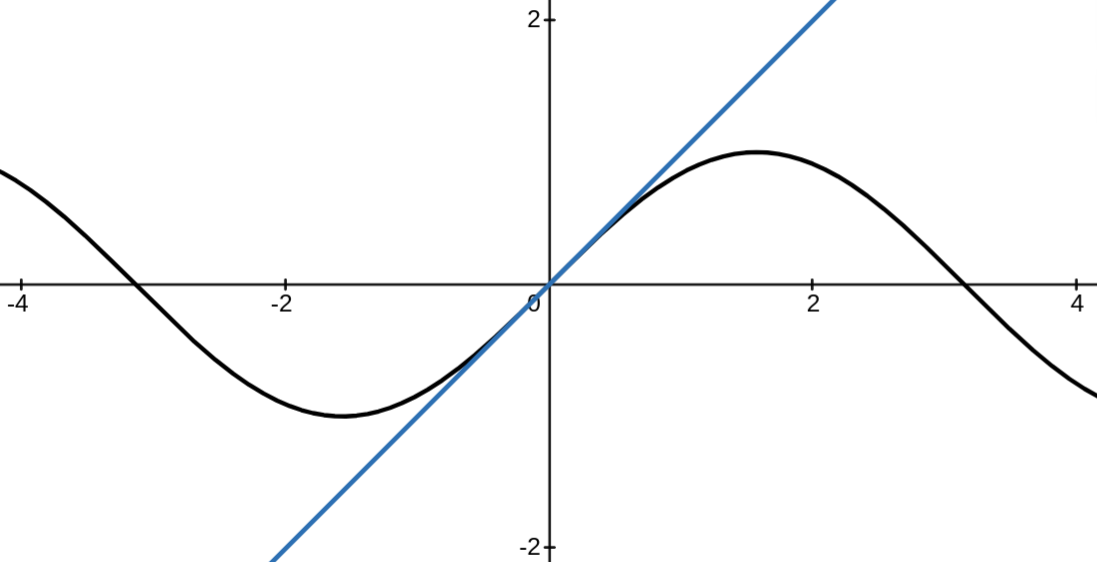
\includegraphics[width=0.7\linewidth]{sin1.png}\]
            \[\sin{x}=x+\bar{\bar{o}}{(x)}\]
            \[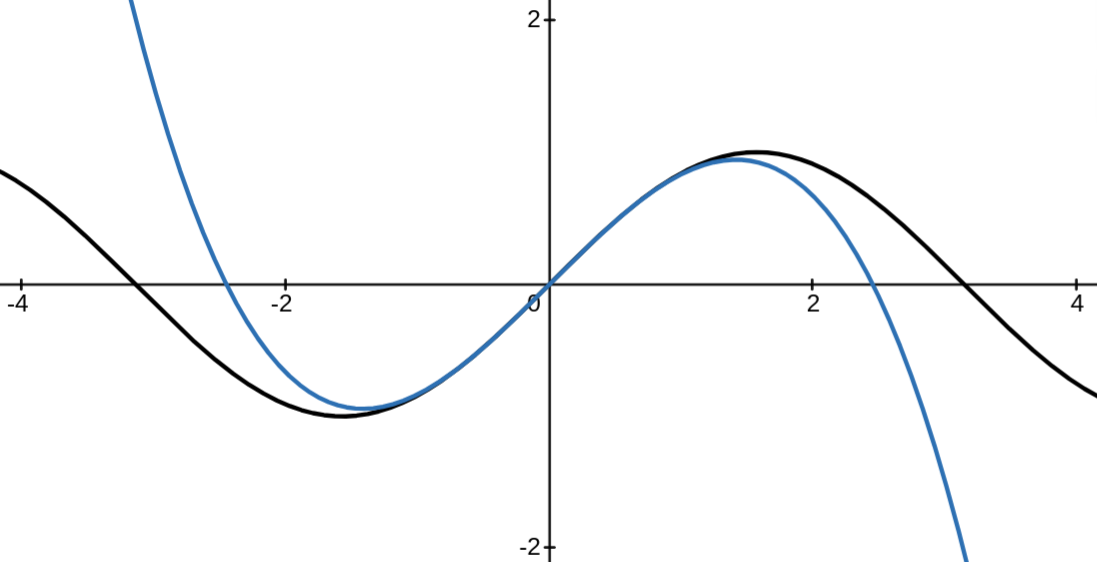
\includegraphics[width=0.7\linewidth]{sin2.png}\]
            \[\sin{x}=x-\frac{x^3}{3!}+\bar{\bar{o}}{(x^3)}\]\\
            \[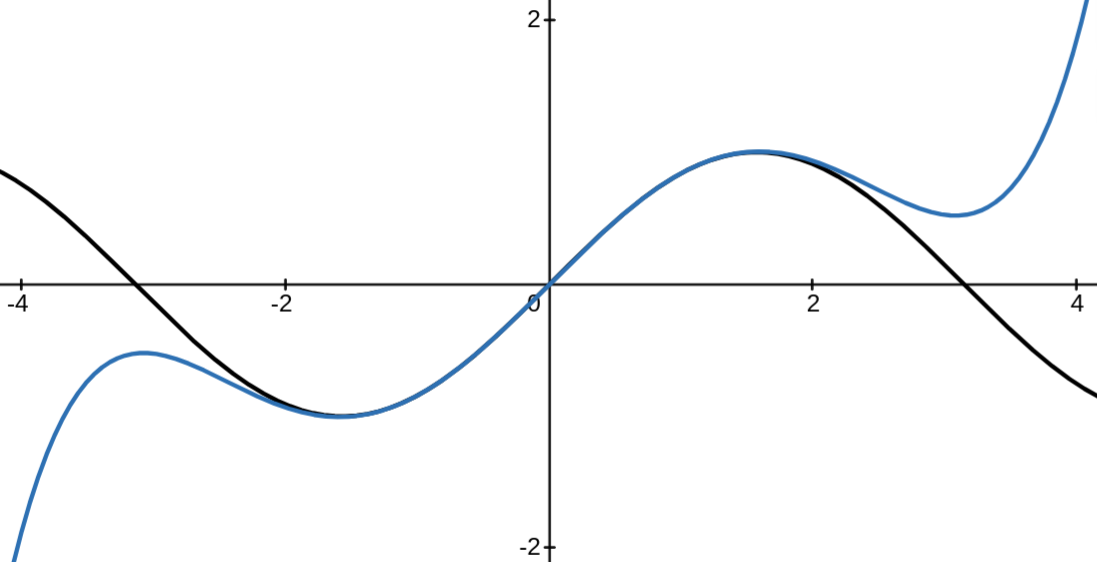
\includegraphics[width=0.7\linewidth]{sin3.png}\]
            \[\sin{x}=x-\frac{x^3}{3!}+\frac{x^5}{5!}+\bar{\bar{o}}{(x^5)}\]\\
            \[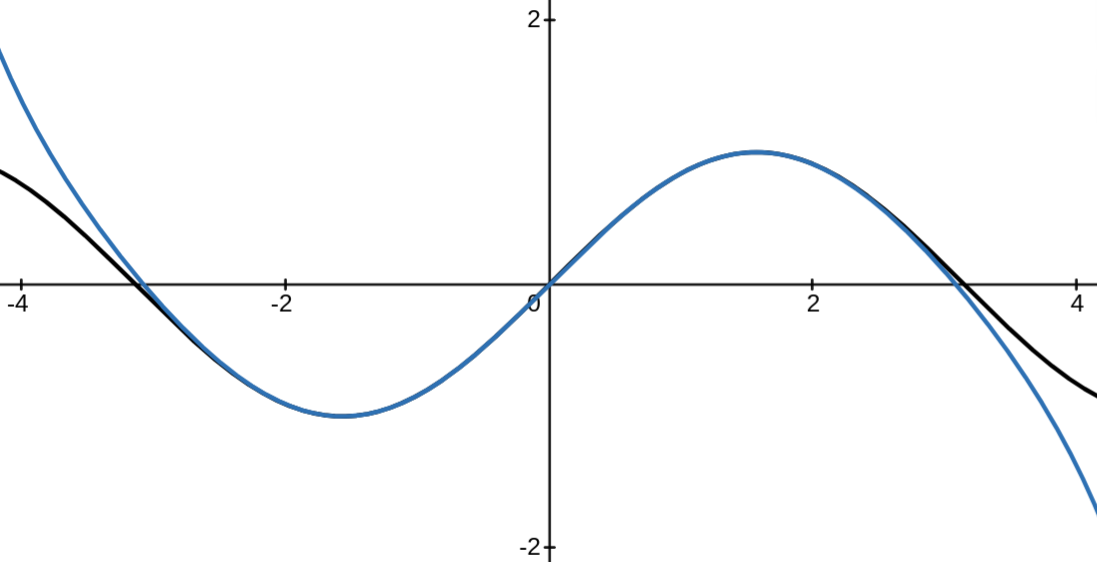
\includegraphics[width=0.7\linewidth]{sin4.png}\]
            \[\sin{x}=x-\frac{x^3}{3!}+\frac{x^5}{5!}-\frac{x^7}{7!}+\bar{\bar{o}}{(x^7)}\]
        \end{example}
        \subsection{Экстремум функции}
        \begin{theorem} (Достаточное условие локального экстремума 1)\\
            Пусть $f(x)\in \mathcal{C}(B(x_0)),\ f(x)\in \mathcal{D}(\mathring{B}(x_0))$. \\
            Если при $x<x_0: f'(x)>0$ или при $x>x_0: f'(x)<0$, то $x_0$ - точка максимума.\\
            Если при $x<x_0: f'(x)<0$ или при $x>x_0: f'(x)>0$, то $x_0$ - точка минимума.
        \end{theorem} 
        \begin{proof}
            По формуле Лагранжа: $f(x)-f(x_0)=f'(c)(x-x_0)$
        \end{proof} 
        \begin{theorem} (Достаточное условие локального экстремума 2)\\
            Пусть $\exists\ f^{(n)}(x_0)\ne 0,\ f^{(k)}(x_0)=0,\ k=1, \dots, n-1$.
            \begin{enumerate}
                \item Если $n=2k+1$, то экстремум нет.
                \item Если $n=2k$, то
                \begin{itemize}
                    \item если $f^{(n)}(x_0)>0$, то $x_0$ точка минимум
                    \item если $f^{(n)}(x_0)<0$, то $x_0$ точка максимума.
                \end{itemize}
            \end{enumerate}
        \end{theorem} 
        \begin{proof}
            \[f(x)=f(x_0)+\frac{f^{(n)}(x_0)}{n!}(x-x_0)^n+\bar{\bar{o}}{(x-x_0)^n},\ x\to x_0\]
            \[\Rightarrow f(x)-f(x_0)=(x-x_0)^n(\frac{f^{(n)}(x_0)}{n!}+\bar{\bar{o}}{(1)})\]
            Заметим, что знак $\frac{f^{(n)}(x_0)}{n!}+\bar{\bar{o}}{(1)}$ совпадает со знаком $f^{(n)}(x_0)$ в некоторой проколотой окрестности $x_0$. Значит,
            \begin{enumerate}
                \item Если $n=2k+1$, то $(x-x_0)^n$ меняет знак при переходе $x$ через точку $x_0 \Rightarrow$ при этом переходе $f(x)-f(x_0)$ тоже меняет свой знак $\Rightarrow x_0$ - не экстремум.
                \item Если $n=2k$, то $(x-x_0)^n$ не меняет знак при переходе $x$ через точку $x_0 \Rightarrow$ если $f^{(n)}(x_0)>0$, то $\forall x \in \mathring{B}(x_0): f(x)-f(x_0)>0 \Rightarrow x_0$ - точка минимума. Аналогично при $f^{(n)}(x_0)<0: x_0$ - точка максимума.
            \end{enumerate}
            
        \end{proof} 
        \subsubsection*{Схема поиска глобального экстремума}
        \begin{enumerate}
            \item Ищем точки интервала $(a,b)$, где $f'(x)=0$ или где ее не существует. 
            \item Находим значение во всех этих точках и значения на концах открезка.
            \item Сравниваем их между собой.
        \end{enumerate}
        \subsection{Выпуклые функции}
        \begin{definition}
            Пусть $f(x)\in \mathcal{C}(I)$. Если $\forall x_1,x_2\in I$ и $\forall x: x_1<x<x_2$:
            \[f(x)\leq \frac{f(x_2)(x-x_1)+f(x_1)(x_2-x)}{x_2-x_1}\]
            то $f(x)$ называется выпуклой вниз. Если выполнено обратное неравенство, то $f(x)$ называется выпуклой вверх. Пример выпуклой вниз функции :
        \end{definition} 
        \begin{center}
            \begin{tikzpicture}[scale=2]
                \draw[->] (-0.5, 0) -- (3.5, 0) node[right] {$x$};
                \draw[->] (0, -0.5) -- (0, 2.5) node[above] {$y$};
                \draw[domain=0.4:3.2,samples=100] plot (\x,{((ln(\x))^2-(0.5*\x)+1.5)});
                \coordinate (x1) at (0.5,0);
                \coordinate (x2) at (3,0);
                \coordinate (y1) at (0.5,1.73);
                \coordinate (y2) at (3,1.2);

                \draw[fill] (x1) circle (1pt) node[below] {$x_1$};
                \draw[fill] (x2) circle (1pt) node[below] {$x_2$};
                \draw[fill] (y1) circle (1pt) node[above right] {$f(x_1)$};
                \draw[fill] (y2) circle (1pt) node[above right] {$f(x_2)$};
                
                \draw[dashed] (x1) -- (y1);
                \draw[dashed] (x2) -- (y2);
                \draw (y1) -- (y2);
            \end{tikzpicture}
        \end{center}
        \begin{theorem} (Достаточное условие выпуклости)\\
            Пусть $f'(x)\in \mathcal{D}(I)$.
            \begin{itemize}
                \item Если $f''(x)>0$, то $f(x)$ выпукла вниз.
                \item Если $f''(x)<0$, то $f(x)$ выпукла вверх.
            \end{itemize}
        \end{theorem} 
        \begin{proof}
            Пусть 
            \[l_1(x)=\frac{f(x_2)(x-x_1)+f(x_1)(x_2-x)}{x_2-x_1}\]
            \begin{multline*}
                f(x)-l_1(x)=\\
                =f(x)\frac{(x-x_1)+(x_2-x)}{x_2-x_1}-\frac{f(x_2)(x-x_1)+f(x_1)(x_2-x)}{x_2-x_1}=\tab[2cm]\\
                \tab[3cm]=\frac{(f(x)-f(x_2))(x-x_1)+(f(x)-f(x_1))(x_2-x)}{x_2-x_1}=\tab[5cm]\\
                \tab[3cm]=\frac{-f'(\xi)(x_2-x)(x-x_1)+f'(\eta)(x-x_1)(x_2-x)}{x_2-x_1}=\\=
                \frac{-f''(\chi)(\xi-\eta)(x-x_1)(x_2-x)}{x_2-x_1}
            \end{multline*}
        \end{proof} 
        \begin{theorem}
            Пусть $f'(x)\in \mathcal{D}(I)$. Если $f''(x)>0\ (f''(x)<0)$, то $\forall x_0\in I$:
            \[f(x)-f(x_0)-f'(x_0)(x-x_0)\geq 0\]
        \end{theorem} 
        \begin{proof}
            Пусть $f(x_0)+f'(x_0)(x-x_0)=l_2(x)$
            \[f(x)-l_2(x)=f'(\xi)(x-x_0)-f'(x_0)(x-x_0)=f''(\eta)(\xi-x_0)(x-x_0)\]
            знаки скобок $(\xi-x_0)$ и $(x-x_0)$ одинаковы, значит $(\xi-x_0)(x-x_0)>0$
        \end{proof} 
        \begin{definition}
            Если $f(x)-l_2(x)$ при проходе через точку $x_0$ меняет знак (разные знаки в левой и правой окрестности), то точка $x_0$ называется точкой перегиба.
        \end{definition}
        \begin{theorem} (Необходимое условие наличия точки перегиба)\\
            Пусть $f''(x)\in \mathcal{C}(B(x_0))$. Если $x_0$ - точка перегиба, то $f''(x_0)=0$.
        \end{theorem}  
        \begin{proof}
            Если $f''(x_0)>0$, то в силу непрерывности $f''(x)>0$ в $B(x_0)$, значит $x_0$ - не точка перегиба. Аналогично для $f''(x_0)<0$.
        \end{proof} 
        \begin{theorem} (Достаточное условие наличия точки перегиба)\\
            Пусть $f''(x)\in \mathcal{C}(I)$. Если $f''(x)$ меняется знак при проходе точки $x_0$, то $x_0$ - точка перегиба.
        \end{theorem} 
        \begin{proof}
            $f(x)-l_2(x)=f''(\eta)(\xi-x_0)(x-x_0)$
        \end{proof} 
        \begin{theorem}
            Пусть $f''(x_0)=0,\ f'''(x_0)\ne 0$. Тогда $x_0$ - точка перегиба.
        \end{theorem} 
        \begin{proof}
            \[f(x)=f(x_0)+f'(x_0)(x-x_0)+\frac{f'''(x_0)}{6}(x-x_0)^3+\bar{\bar{o}}{((x-x_0)^3)}\] 
            Тогда
            \[f(x)-l_2(x)=(x-x_0)^3(\frac{f'''(x_0)}{6}+\bar{\bar{o}}{(1)})\]
        \end{proof} 
        \begin{definition}
            Если при $x\to a-0\ (x\to a+0): f(x)\to \pm \infty$, то прямая $x=a$ называется вертикальной асимптотой.
        \end{definition} 
        \begin{definition}
            Если при $x\to +\infty (x\to -\infty): (f(x)-kx-b)\to 0$, то прямая $y=kx+b$ называется наклонной асимптотой.
        \end{definition} 
        \begin{theorem}
            Прямая $y=kx+b$ является наклонной асимптотой графика функции $f(x) \Leftrightarrow \exists \lim\limits_{x\to +\infty}\frac{f(x)}{x}=k,\ \exists \lim\limits_{x\to +\infty}(f(x)-kx)$, аналогично к $-\infty$.
        \end{theorem} 
        \begin{theorem} (Неравенство Йенсена)\\
            Пусть $f(x)$ выпукла вверх (вниз) в каждой точке $I$. Пусть $\forall i: \alpha_i>0,\ \sum\limits_{i=1}^{n}\alpha_i=1$. Тогда $\forall x_i \subset I$:
            \[f(\sum\limits_{i=1}^{n}\alpha_i x_i) \geq \sum\limits_{i=1}^{n}\alpha_i f(x_i)\]
        \end{theorem} 
        \begin{proof}
            Индукция по $n$. Если $n=1$ - очев. Для $n=2$ так как $f(x)$ - выпукла вверх: 
            \[f(\alpha_1 x_1+\alpha_2 x_2)\geq \alpha_1 f(x_1)+\alpha_2 f(x_2)\]
            Пусть верно для $n$. Тогда пользуясь неравенством для $n=1$ и $n=2$ получим:
            \begin{multline*}
                f(\sum\limits_{i=1}^{n+1}\alpha_i x_i)=f(\alpha_{n+1}x_{n+1}+\sum\limits_{i=1}^{n}\alpha_i x_i)=\\
                =f(\alpha_{n+1}x_{n+1}+\sum\limits_{i=1}^{n}\alpha_i \cdot \sum\limits_{i=1}^{n}(\frac{\alpha_i}{\sum\limits_{i=1}^{n}\alpha_i}\cdot x_i))\geq\tab[5cm]\\
                \geq \alpha_{n+1} f(x_{n+1})+\sum\limits_{i=1}^{n}\alpha_i\cdot f(\sum\limits_{i=1}^{n}\frac{\alpha_i}{\sum\limits_{i=1}^{n}\alpha_i} x_i)\geq\\
                \tab[5cm]\geq \alpha_{n+1} f(x_{n+1})+\sum\limits_{i=1}^{n}\alpha_i(\sum\limits_{i=1}^{n}\frac{\alpha_i}{\sum\limits_{i=1}^{n}\alpha_i}\cdot f(x_i))=\\
                =\alpha_{n+1}f(x_{n+1})+\sum\limits_{i=1}^{n}\alpha_i f(x_i)=\sum\limits_{i=1}^{n+1}\alpha_i f(x_i)
            \end{multline*}
        \end{proof} 
        \begin{statement}
            (Неравенство между средним арифметическим и средим геометрическим)
            \[\frac{1}{n}\sum\limits_{k=1}^{n}x_k\geq \sqrt[n]{\prod\limits_{k=1}^{n}x_k}\]
        \end{statement}
        \begin{proof}
            $f(x)=\ln{x},\ f''(x)=-\frac{1}{x^2}<0$ - выпукла вверх. Тогда
            \[\ln({\sum\limits_{k=1}^{n}\frac{1}{n}})\geq \frac{1}{n} \sum\limits_{k=1}^{n}\ln{x}=\ln({\prod\limits_{i=1}^{n}x_k^{\frac{1}{n}}})\]
            Взяв $\exp$ от обеих частей, получим искомое неравенство.
        \end{proof} 
        \begin{statement}
            (Неравенство Юнга)\\
            $\forall a,b<0,\ \forall p,q>1: \frac{1}{p}+\frac{1}{q}=1$. Тогда 
            \[ab\leq \frac{a^p}{p}+\frac{b^q}{q}\]
        \end{statement}
        \begin{proof}
            Воспользуемся неравенством Йенсена для логарифма:
            \[\ln({\frac{1}{p}\cdot x_1+\frac{1}{q}\cdot x_2})\geq \frac{1}{p}\cdot \ln{x_1}+\frac{1}{q}\cdot \ln{x_2}\]
            $x_1=a^p,\ x_2=b^q$. Тогда
            \[\ln{\frac{a^p}{p}+\frac{b^q}{q}}\geq \ln{a}+\ln{b}=\ln{ab}\]
        \end{proof} 
        Взяв $\exp$ от обеих частей, получим искомое неравенство.
\end{document}